\clubpenalty100000000
\widowpenalty100000000
\documentclass[xetex, svgnames, 12pt]{scrartcl}

\usepackage{xeCJK}
\setCJKmainfont{BabelStone Han}
\usepackage{multicol}
\usepackage{enumitem}
\usepackage{setspace}
\usepackage[left=2.5cm, right=2.5cm, top=3cm, bottom=3cm]{geometry}
% XeLaTeX settings
\usepackage{xltxtra,polyglossia}
\setmainfont[Mapping=tex-text,Scale=1.0]{FreeSerif}
\setsansfont[Mapping=tex-text,Scale=1.0]{FreeSans}
\setmonofont{FreeMono}
\setmainlanguage{english}
\usepackage{makecell}
\usepackage{tabu}



\newfontfamily\tibetan{Tibetan Machine Uni}
\newfontfamily\sil{Charis SIL}
% Text styles
\newcommand\Bod[1]{\tibetan\textup{#1}}

\newcommand{\textunderset}[2]{\begin{tabular}[t]{@{}c@{}}#2\\[-0.3em]\scriptsize#1\end{tabular}}
\newcommand{\textoverset}[2]{\begin{tabular}[b]{@{}c@{}}\scriptsize#1\\[-0.38em]#2\end{tabular}}
\newcommand{\textoversetlarge}[2]{\begin{tabular}[b]{@{}c@{}}\scriptsize#1\\[-0.2em]#2\end{tabular}}



\newfontfamily\burm{Padauk}
\usepackage{scrlayer-scrpage}
\usepackage[
    colorlinks,
    urlcolor=black,
    linkcolor=black,
    citecolor=CornflowerBlue,
    filecolor=black,
    linktocpage=true,
    %dvipdfm
    ]{hyperref}

% more packages needed
\usepackage{tikz-cd}
\usepackage{amsfonts}
\usepackage{amsmath}
\usepackage{amssymb}
\usepackage{xcolor, color, colortbl, multirow}
% biblatex is used for bibtex rendering, style author-year
\usepackage[
    backend=bibtex,
    bibstyle=authoryear,
    giveninits=true,
    ibidtracker=strict,
    isbn=false,doi=false,url=false,
    labelnumber=true,
    loccittracker=strict,
    maxbibnames=10,
    maxcitenames=2,
    natbib=true,
    opcittracker=strict,
    sortcites=true,
    sorting=nyt,
    style=authoryear-ibid,
    alldates=terse,
    terseinits=false
    ]{biblatex}

\renewcommand*{\nameyeardelim}{\addspace}
\DeclareFieldFormat{postnote}{#1}
\DeclareFieldFormat{multipostnote}{#1}

\renewcommand\bibfont{\footnotesize}


% pagestyle settings
\pagestyle{scrheadings}
\ihead{%Hill
}
\chead{Chinese Dictionary}
\ohead{}
\ifoot{}
\cfoot{\pagemark}
\ofoot{}

\bibliography{asia}
\usepackage{setspace}
\usepackage{tabularx}
\usepackage{adjustbox}
\usepackage[]{tikz}
\graphicspath{{images/}{../images/}}

\usetikzlibrary{calc,arrows,positioning,shapes}

\newcommand{\SET}[1]  {\ensuremath{\mathcal{#1}}}
\newcommand{\MAT}[1]  {\ensuremath{\boldsymbol{#1}}}
\newcommand{\VEC}[1]  {\ensuremath{\boldsymbol{#1}}}
\newcommand{\Video}{\SET{V}}
\newcommand{\video}{\VEC{f}}
\newcommand{\track}{x}
\newcommand{\Track}{\SET T}
\newcommand{\LMs}{\SET L}
\newcommand{\lm}{l}
\newcommand{\PosE}{\SET P}
\newcommand{\posE}{\VEC p}
\newcommand{\negE}{\VEC n}
\newcommand{\NegE}{\SET N}
\newcommand{\Occluded}{\SET O}
\newcommand{\occluded}{o}
%\definecolor{amazongreen}{cmyk}{0.83,0.24,0,0.12}
\definecolor{blue}{rgb}{0.0, 0.0, 0.55}
\definecolor{green}{rgb}{0.0, 0.5, 0.0}
\definecolor{red}{rgb}{0.75, 0.0, 0.2}
\definecolor{violet}{RGB}{153,153,255}
\definecolor{antiquewhite}{rgb}{0.98, 0.92, 0.84}
\definecolor{amazongreen}{RGB}{0,153,153}

%\newfontfamily\burm{Padauk}
\newfontfamily\tib{Tibetan Machine Uni}


%Define boxes

\tikzstyle{startstop} = [rectangle, rounded corners, minimum width=4.2cm, minimum height=1cm,text centered, draw=amazongreen, text=white, fill=red!30]
\tikzstyle{process} = [rectangle, minimum width=4.2cm, minimum height=1cm, text centered, draw=amazongreen, fill=orange!30, text=white]
%\tikzstyle{decision} = [diamond, minimum width=3cm, minimum height=1cm, text centered, draw=black, fill=green!30]
\tikzstyle{decision} = [rectangle, rounded corners,minimum width=4cm, minimum height=1cm, text centered, text width=3cm, text=white, fill=amazongreen]

% Draw a video
\newlength{\FSZ}
\newcommand{\drawvideo}[3]{% [0 0.25 0.5 0.75 1 1.25 1.5]
   \noindent\pgfmathsetlength{\FSZ}{\linewidth/#2}
   \begin{tikzpicture}[outer sep=0pt,inner sep=0pt,x=\FSZ,y=\FSZ]
   \draw[color=amazongreen!50!black] (0,0) node[outer sep=0pt,inner sep=0pt,text width=\linewidth,minimum height=0] (video) {\noindent#3};
   \path [fill=amazongreen!50!black,line width=0pt] 
     (video.north west) rectangle ([yshift=\FSZ] video.north east) 
    \foreach \x in {1,2,...,#2} {
      {[rounded corners=0.6] ($(video.north west)+(-0.7,0.8)+(\x,0)$) rectangle +(0.4,-0.6)}
    }
;
   \path [fill=amazongreen!50!black,line width=0pt] 
     ([yshift=-1\FSZ] video.south west) rectangle (video.south east) 
    \foreach \x in {1,2,...,#2} {
      {[rounded corners=0.6] ($(video.south west)+(-0.7,-0.2)+(\x,0)$) rectangle +(0.4,-0.6)}
    }
;
   \foreach \x in {1,...,#1} {
     \draw[color=amazongreen!50!black] ([xshift=\x\linewidth/#1] video.north west) -- ([xshift=\x\linewidth/#1] video.south west);
   }
   \foreach \x in {0,#1} {
     \draw[color=amazongreen!50!black] ([xshift=\x\linewidth/#1,yshift=1\FSZ] video.north west) -- ([xshift=\x\linewidth/#1,yshift=-1\FSZ] video.south west);
   }
   \end{tikzpicture}
}

\title{A dictionary of Chinese characteres in transliteration}
\author{Nathan W. Hill}
\begin{document}
\maketitle
\begin{abstract}
\noindent 
\end{abstract}

%%%%%%%%%%%%%%%%%%%%%%%%%%%%%%%%%%%%%%%%%%%%%%%%%%%%%%%%%%%%%%%%%%%%%%%%%%%%%%%%%%%%%%%%%%%%%%%%

\section{Semantic components}
\begin{multicols}{3}
\begin{itemize}[noitemsep]
    \item 辛 acr(is)
    \item 黹 acu(laria)
    \item 尚 
    %(shàng) - 
    adhuc 
    %(still, yet, even, still more) 
    \item 田 ager 
    \item 白 alb(us) 
    \item 高 alt(us) 
    \item 辵 amb(ulo)
    \item 黽 amph(ibium)
    \item 古 
    %(gǔ) - 
    antiqu(us) 
    %(ancient, old) 
    \item 弓 
    %(gōng) - 
    arc(us) 
    %(bow) 
    \item 水 aq(ua) 
    \item 耒 
    %(lěi) -
    aratr(um) 
    %(plow) 
    \item 木 arb(or) 
    \item 耳 aur(is) 
    \item 鳥 av(is)
    \item 竹 bamb(us)
    \item 須 barb(a)
    \item \symbol{"268DE}
barbil(ia)
    \item 豸 best(ia) 
    \item 牛 bos 
    \item 尸 cadaver
    \item 犬 can(is) 
    \item 首 cap(ut) 
    \item 匚 caps(a)
    \item 肉 carn(is) 
    \item 厂 caut(es)
    \item 穴 cav(us) 
    \item 鹿 cerv(us) 
    \item 止 cess(o)
    \item 申 tend(o)
    \item 單 cicad(a)
    \item 雚 ciconia (in 飌)
    \item 丹 cinnabar(is) (in 彤)
    \item 囗 cla(usum) 
    \item 尢 claud(us)
    \item 思 
    %(sī) - 
    cogit(o) 
    %(to think, to ponder) 
    \item 丘/丠 coll(is)
    \item 貝 conch(a)
    \item 心 cor 
    \item 革 
    %(gé) - 
    cori(um) 
    %(leather, to reform, to revolutionize) 
    \item 角 corn(u) 
    \item 身 corp(us)
    \item 髟 crin(is) 
    \item 刀 cult(er)
    \item 走 curr(o)     
    \item 鬼 daemon 
    \item 欠 dehab(eo)
    \item 去 depart(ire)
    \item 齒 (dens), dent(is)
    \item 又 dextr(a)
    \item 言 dic(o) 
    \item 音 son(us)
    \item 寸 digit(us)
    \item 舍 dom(us) 
    \item 龍 (draco), dracon(is) (in 龏)
    \item 甘 dulc(is) (in 甞)
    \item 食 ed(o) 
    \item 行 eo 
    \item 象 
    %(xiàng) - 
    elephant(us) 
   \item 馬 equ(us)
   \item 出 ex(ire)
   \item 頁 fac(ies)
   \item 女 fem(ina) 
   \item 攴 fer(io) 
   \item 勹 flect(o)
   \item 子 fili(us) 
   \item 臤 firm(us)
   \item 川 fluvi(us)
   \item 田 forn(us) (only in 盧)
   \item \symbol{"2201C} fov(ere) (only in 筑)
   \item 黃 \makebox[0pt][l]{galb(inus) (only in 黈?)}  
   \item 仌 glac(ies)    
   \item 玉 gem(ma)
   \item 屮 germ(en)
   \item 癶 grad(us)
   \item 禾 gran(um) 
   \item 犛 \makebox[0pt][l]{(bos) grunn(iens)} \\ (only in 斄)
   \item 旨 gust(us) (in 嘗)
   \item 戈 hallebard(a) 
   \item 殳 hast(a)
   \item 艸 herb(a) 
   \item 人 hom(o) 
   \item 矛 iacul(um)
   \item 火 ign(is) 
   \item 疒 infirm(itas)
   %(recovered from entry usage)
   \item 兮 io 
   \item 敕 iuss(us)
   \item 石 lap(is)
   \item 匸 latebr(a)
   \item 广 lax(us) 
   \item 斤 libra 
   \item 舌 lingu(a)
   \item 巾 lint(eum) 
   \item 月 luna 
   \item 光 lux
   \item 大 magn(us) 
   \item 歹 mal(us) 
   \item 手 man(us) 
   \item 男 masc(ulus) 
   \item 午 meridi(es)
   \item 金 met(allum)
   \item 黍 \makebox[0pt][l]{mil(ium) (only in 黎?)}
   \item 牙 molar(is dens)
    \item 山 mon(s)
   \item 鼠 rod(entia)
    \item 鼻 nas(um)
    \item 网 nass(a) 
    \item 非 ne
    \item 舟 nav(is) 
    \item 黑 niger 
    \item 旡 non 
    \item 監 observ(o) 
    \item 舛 obs(isto) 
    \item 目 ocul(us)
    \item 鬲 olla
    \item 米 oryz(a) 
    \item 口 (os,) or(is)
    \item 骨 (os,) oss(is) 
    \item 戶 ost(ium)
    \item 羊 ov(is)
    \item 帛 pann(us)
    \item 幺 parv(us) 
    \item 亠 pav(ilio)
    \item 步 pass(us)
    \item 隹 passer
    \item 足 (pes,) ped(is) 
    \item 皮 pell(is) (in 皽)
    \item 毛 pil(us)
    \item 聿 pincern(a) 
    \item 魚 pis(cis) 
    \item 民 pleb(s)
    \item 羽 plum(a)
    \item 雨 pluv(ia) 
    \item 豕 porc(us) 
    \item 門 port(a) 
    \item 可 poss(um) 
    \item 玄 profund(us) 
    \item 卜 prognosc(ere) (in 鼑)
    \item 廴 progred(ior) (in 廷)
    \item 鬥 pugn(a)
    \item 方 quadr(us)
    \item 支 ram(us) 
    \item 赤 ruf(us) 
    \item 矢 sagit(ta)
   \item 鹵 sal(is)
   \item 血 sangu(is)
   % \item 章 sculp(ō) (in 贛)
    \item 戊 secur(is) (in 戚)
    \item 片 segm(entum)
    \item 老 sen(ex)
    \item 糸 ser(icum)
    \item 虫 serp(ens)
    \item 林 %(lín) - 
    silv(a) %(forest)
    \item 日 sol 
    \item 卩 sign(o) 
    \item 㝱 
    %(méi) - 
    somn(ium)
    \item 音 son(us)
    \item 示 spirit(us) 
    \item 立 sto
    \item 鼓 tabur (only in 鼛?)
    \item 宀 tect(um) 
    \item 瓦 teg(ula) 
    \item 亯 templ(um) (in 䈞)
    \item 丮 ten(eo)
    \item 申 tend(o)
    \item 土 terr(a) 
    \item 龠 tibia 
    \item 虍 
    %(hū) - 
    tigr(is) 
    %(tiger) 
    \item 鼎 trip(us)
    \item 斗 
    %(dǒu) - 
    trull(a) 
    %(dipper, ladle) 
    \item 爾 
    tu 
    %(you, your) 
    \item 阜 tum(ulus) 
    \item 壴 
    %(zhù) - 
    tympan(um) 
    \item 邑 urb(s) 
    \item 熊 urs(us)
    \item 箕 vann(us)
    \item 皿 vas(um) 
    \item 車 vehic(ulum) 
    \item 來 veni(ō)
    \item 胃 ventri(culus)
    \item 風 vent(us)
    \item 衣 vest(imentum) 
    \item 㫃 vex(illum) 
    \item 里 vic(us) 
    \item 見 vid(eo) 
    \item 酉 vin(um)
    \item 力 virt(us)
\end{itemize}
\end{multicols}

\section{Semantics still to alphabetize}
% none currently



\section{The dictionary itself}

\subsection{-ay}
\begin{multicols}{2}
\paragraph{\textoversetlarge{18-01}{\huge{可}}}
{\Large{qay}}, 
%ke3	
\textit{khaX};	%0001a
柯	%ke1	
{\large{{\textsuperscript{arb·}}
qay}}, 
\textit{ka};		%0001d
笴	%gan3	
{\large{\textsuperscript{bamb:}qay}},
\textit{kanX},		%0001e
%笴	%ge3	
\textit{kaX};		%0001e
河	%he2	
{\large{\textsuperscript{aq·}qay}},
\textit{ḫa};		%0001g
苛	%ke1	
{\large{\textsuperscript{herb:}qay}},
\textit{ḫa};		%0001i
呵	%he1	
{\large{\textsuperscript{or·}qay}},
\textit{ḫa};		%0001j
訶	%he1	
{\large{\textsuperscript{dic·}qay}},
\textit{ḫa};		%0001k
阿	%e1	
{\large{\textsuperscript{tum·}qay}},
\textit{{\sil{ꞏ}}a};		%0001m
㫊	%yi3	
\textit{{\sil{ꞏ}}aX},		%0001n
%㫊	%yi3	
\textit{{\sil{ꞏ}}ieX};		%0001n
\begin{itemize}[noitemsep]
\begin{spacing}{0.7} 

\item 
{\Large{何}}	%he2	
{\large{\textsuperscript{hom·}qay}}
= 
{\large{g\textoverset{a}{a}y}},
\textit{ḫa},		%0001f
%何	%he2	
\textit{ḫaX};		%0001f
荷	%he2	
{\large{{\textsuperscript{bamb:}}g\textoverset{a}{a}y}}, 
\textit{ḫa};		%0001o
    \item 
{\Large{哥}}	%ge1	
{\large{qay:qay}} = {\large{k\textoverset{a}{a}y}},
\textit{ka};		%0001p
歌	%ge1	
{\large{k\textoverset{a}{a}}y{\textsuperscript{·dehab}}}, 
\textit{ka};		%0001q
謌	%ge1	
{\large{{\textsuperscript{dic·}}k\textoverset{a}{a}y}}, 
\textit{ka};		%0001r
\item
{\Large{奇}}	%qi2	
{\large{\textsuperscript{magn:}qay}}
= {\large{q\textoverset{b}{a}y}},
\textit{gie},		%0001s
%奇	%ji1	
\textit{kie};		%0001s
琦	%qi2	
{\large{\textsuperscript{gem·}q\textoverset{b}{a}y}},
\textit{gie};		%0001t
騎	%qi2	
{\large{\textsuperscript{equ·}q\textoverset{b}{a}y}},
\textit{gie};		%0001u
錡	%qi2	
{\large{\textsuperscript{met·}q\textoverset{b}{a}y}},
\textit{gie},		%0001v
	%qi2	
\textit{gieX},		%0001v
%錡	%yi3	
\textit{ṅieX};		%0001v
寄
{\large{\textsuperscript{tect:}q\textoverset{b}{a}y}},
	%ji4	
\textit{kieH};		%0001x
掎	%ji3	
{\large{\textsuperscript{man·}q\textoverset{b}{a}y}},
\textit{kieX};		%0001y
畸	%ji1	
{\large{\textsuperscript{ag·}q\textoverset{b}{a}y}},
\textit{kie};		%0001z
羇	%ji1	
\textit{kie};		%0001a'
綺	%qi3	
{\large{\textsuperscript{ser·}q\textoverset{b}{a}y}},
\textit{khieX};		%0001b'
踦	%qi1	
{\large{\textsuperscript{ped·}q\textoverset{b}{a}y}},
\textit{khie},		%0001c'
%踦	%ji3	
\textit{kieX},		%0001c'
%踦	%yi3	
\textit{ṅieX};		%0001c'
攲	%qi1	
{\large{q\textoverset{b}{a}y\textsuperscript{·ram}}},
\textit{khie};		%0001d'
%攲	%ji1	
\textit{kie};		%0001d'
觭	%ji1	
{\large{\textsuperscript{corn·}q\textoverset{b}{a}y}},
\textit{khie};		%0001e'
倚	%yi3	
{\large{\textsuperscript{hom·}q\textoverset{b}{a}y}},
\textit{{\sil{ꞏ}}ieX};		%0001f'
椅	%yi1	
{\large{\textsuperscript{arb·}q\textoverset{b}{a}y}},
\textit{{\sil{ꞏ}}ie};		%0001g'
猗	%e1	
{\large{\textsuperscript{can·}q\textoverset{b}{a}y}},
\textit{{\sil{ꞏ}}aX},	%0001h'
%猗	%yi1	
\textit{{\sil{ꞏ}}ie},		%0001h'
%猗	%yi3	
\textit{{\sil{ꞏ}}ieX};		%0001h'
輢	%yi3	
{\large{\textsuperscript{vehic·}q\textoverset{b}{a}y}},
\textit{{\sil{ꞏ}}ieX};	%0001i'
陭	%yi1	
{\large{\textsuperscript{tum·}q\textoverset{b}{a}y}},
\textit{{\sil{ꞏ}}ie}.		%0001j'
\end{spacing}
\end{itemize}

\paragraph{\textoversetlarge{18-03}{\huge{羅}}}
%luo2	
{\large{ray}},
\textit{la};	%la	0006a
蘿	%luo2	
{\large{{\textsuperscript{herb:}}ray}},
\textit{la}.	%la	0006b

18-03/1238a 羈 
{\large{{\textsuperscript{herb:}}ray}},
\textit{kje}

18-03/07-33/1240c 
{\large{{\textsuperscript{herb:}}ray}},
買 \textit{meaX}

18-03/07-33/1240e 
{\large{{\textsuperscript{herb:}}ray}},
賣 \textit{meaH}

18-03/18-10/0006a 羅 
{\large{{\textsuperscript{herb:}}ray}},
\textit{la}

18-03/18-10/0006b 蘿 
{\large{{\textsuperscript{herb:}}ray}},
\textit{la}

18-03/18-10/0024a 罹 
{\large{{\textsuperscript{herb:}}ray}},
\textit{lje}

\begin{itemize}[noitemsep]
    \item 
{\Large{罷}}	%ba4	
\textit{beaX};	%beaX	0026a
%罷	%pi2	
\textit{bie};	%bje	0026a
羆	%pi2	
\textit{pie}.	%pje	0026b
\end{itemize}

Baxter \& Sagart (personal communication 11 April 2017) combine Schuessler's 07-33, 18-03, 18-10, and 18-17.

\paragraph{\textoversetlarge{18-04}{\huge{加}}}
{\large{kay}},
%加	%jia1	
\textit{kae};	%kae	%0015a
枷	%jia1	
{\large{{\textsuperscript{arb·}}kay}},
\textit{kae};	%kae	%0015c
%枷	%jia1	
\textit{kaeH};	%kaeH	%0015c
珈	%jia1	
{\large{{\textsuperscript{gem·}}kay}},
\textit{kae};	%kae	%0015d
駕	%jia4	
{\large{kay{\textsuperscript{:equ}}}},
\textit{kaeH};	%kaeH	%0015e
嘉	%jia1	
{\large{{\textsuperscript{tympan:}}kay}},
\textit{kae};	%kae	%0015g
哿	%ge3	
{\large{kay{\textsuperscript{:poss}}}},
\textit{kaX};	%kaX	%0015i
賀	%he4	
{\large{kay{\textsuperscript{:conch}}}},
\textit{ḫaH};	%haH	%0015j





\paragraph{\textoversetlarge{18-05}{\huge{我}}}
%wo3	
{\Large{ṅay}}, 
\textit{ṅaX};		%0002a
俄	%e2	
{\large{{\textsuperscript{hom·}}
ṅay}}, 
\textit{ṅa};		%0002h
娥	%e2	
{\large{{\textsuperscript{fem·}}
ṅay}},
\textit{ṅa;}		%0002i
峨	%e2	
{\large{{\textsuperscript{mon·}}
ṅay}},
\textit{ṅa};		%0002k
睋	%e2	
{\large{{\textsuperscript{ocul·}}
ṅay}},
\textit{ṅa};		%0002l
莪	%e2	
{\large{{\textsuperscript{herb:}}ṅay}},
\textit{ṅa};		%0002m
誐	%e2	
{\large{{\textsuperscript{dic·}}ṅay}},
\textit{ṅa};		%0002n
餓	%e4	
{\large{{\textsuperscript{ed·}}ṅay}},
\textit{ṅaH};		%0002o
鵝	%e2	
{\large{ṅay{\textsuperscript{·av}}}},
\textit{ṅa};		%0002p
鵞	%e2	
{\large{ṅay{\textsuperscript{:av}}}},
\textit{ṅa};		%0002p
蛾	%e2	
{\large{{\textsuperscript{serp·}}ṅay}},
\textit{ṅa},		%0002q
	%yi3	
\textit{ṅieX}.\footnote{Were it not for the one reading \textit{ṅieX}, 我 {\large{ṅay}} could have been written {\large{ṅ\textoverset{a}{a}y}}.}		
\begin{itemize}[noitemsep]
\begin{spacing}{0.7} 
    \item 
{\Large{義}}	%yi4	
{\large{{\textsuperscript{ov:}}ṅay}} =
{\large{ṅ\textoverset{b}{a}y}},
\textit{ṅieH};		%0002r
儀	%yi2	
{\large{{\textsuperscript{hom·}}ṅ\textoverset{b}{a}y}},
\textit{ṅie};	%0002u
議	%yi4	
{\large{{\textsuperscript{dic·}}ṅ\textoverset{b}{a}y}},
\textit{ṅieH};		%0002v
蟻	%yi3	
{\large{{{\textsuperscript{serp·}}ṅ\textoverset{b}{a}y}}},
\textit{ṅieX};		%0002x
\begin{itemize}[noitemsep]
    \item 
{\Large{羲}}	%xi1	
{\large{{\textsuperscript{io·}}ṅ\textoverset{b}{a}y}} = 
{\large{ṅh\textoverset{b}{a}y}},
\textit{hie};		%0002y
犧	%xi1	
{\large{ṅh\textoverset{b}{a}y}},
\textit{hie}.		%0002z
\end{itemize}
\end{spacing}
\end{itemize}



\paragraph{\textoversetlarge{18-06}{\huge{宜}}}
%宜	%yi2	
{\large{ṅay}},
\textit{ṅie};	%ngje	0021a
誼	%yi4	
{\large{{\textsuperscript{dic·}}ṅay}},
\textit{ṅieH}.	%ngjeH	0021h

\paragraph{\textoversetlarge{18-07}{\huge{䖒}}}	%xi1	
{\large{ṅay}},
\textit{hie};	%xje	0022a
戲	%xi4	
{\large{{ṅay{\textsuperscript{·hallebard}}}}},
\textit{hieH}. 	%xjeH	0022b

Acc. to Wiktionary to be united with 虍 xu



\paragraph{\textoversetlarge{18-08}{\huge{多}}}
{\large{lay}},
%duo1	
 \textit{ta}		%0003a
痑	%duo3	
{{\textsuperscript{infirm·}}\large{lay}}, 
\textit{taH},		%0003d
%痑	%duo3	
\textit{tha};		%0003d
奓	%zha1	
{{\textsuperscript{magn:}}\large{lay}},
\textit{ṭae};		%0003e
㗬	%cha1	
{{\textsuperscript{adhuc:}}
\large{lay}},
\textit{ṭhae};		%0003f
恀	%shi4	
{{\textsuperscript{cor·}}
\large{lay}},
\textit{cieX};		%0003h
侈	%chi3	
{{\textsuperscript{hom·}}
\large{lay}},
\textit{chieX};		%0003i
拸	%chi3	
{{\textsuperscript{man·}}
\large{lay}},
\textit{ṭhieX};		%0003j
哆	%chi3	
{{\textsuperscript{or·}}
\large{lay}},
\textit{chiaeX};		%0003k
誃	%chi2	
{{\textsuperscript{dic·}}
\large{lay}},
\textit{ḍie},		%0003l
%誃	%chi3	
\textit{chieX};		%0003l
趍	%chi2	
{{\textsuperscript{curr·}}
\large{lay}},
\textit{ḍie};		%0003m
陊	%duo4	
{{\textsuperscript{tum·}}
\large{lay}},
\textit{ḍieX};		%0003o
移	%yi2	
{{\textsuperscript{gran·}}
\large{lay}},
\textit{yie},	%0003q
%移	%yi4	
\textit{yieH};		%0003q
迻	%yi2	
{{\textsuperscript{amb·}}
\large{lay}},
\textit{yie};	%0003r
㢋	%chi3	
{{\textsuperscript{lax·}}
\large{lay}},
\textit{chieX}.	%0003t



\paragraph{\textoversetlarge{18-09}{\huge{它}}}
{\large{lay}},
\textit{tha};		%0004a
㐌	%ta1	
\textit{tha};		%0004f
\begin{itemize}[noitemsep]
\item 
佗	%tuo1	
{{\textsuperscript{hom·}}
\large{lay}},
\textit{da};		%0004h
%佗	%tuo1	
\textit{thaH};		%0004h
拕	%tuo1	
{{\textsuperscript{man·}}
\large{lay}},
\textit{tha},		%0004i
%拕	%tuo1	
\textit{thaH};		%0004i
紽	%tuo2	
{{\textsuperscript{ser·}}
\large{lay}},
\textit{da};		%0004j
沱	%tuo2	
{{\textsuperscript{aq·}}
\large{lay}},
\textit{da};		%0004k
蛇	%yi2	
{{\textsuperscript{serp·}}
\large{lay}},
\textit{yie},		%0004l
%蛇	%she2	
\textit{jiae};		%0004l
鉈	%shi1	
{{\textsuperscript{met·}}
\large{lay}},
\textit{śiae};		%0004m
\end{itemize}
匜	%yi2	
\textit{yie}	%0004n
\begin{itemize}[noitemsep]
    \item 
也	
{\large{lay}},
%ye3	
\textit{yaeX};		%0004g
訑	%yi2	
{{\textsuperscript{dic·}}\large{lay}}, 
\textit{tha},		%0004q
%訑	%yi2	
\textit{thwa},		%0004q
%訑	%yi2	
\textit{yie};		%0004q
迆	%yi2	
{\large{{\textsuperscript{amb·}}lay}}, 
\textit{yie};		%0004r
酏	%yi2	
{\large{{\textsuperscript{vin·}}lay}}, 
\textit{yie};		%0004s
池	%chi2	
{\large{{\textsuperscript{aq·}}lay}}, 
\textit{ḍie};		%0004t
竾	%chi2	
{\large{lay}}, 
\textit{ḍie};		%0004v
馳	%chi2	
{\large{{\textsuperscript{equ·}}lay}}, 
\textit{ḍie};		%0004x
杝	%zhi4	
{\large{{\textsuperscript{arb·}}lay}}, 
\textit{ḍieX},		%0004y
%杝	%yi2	
\textit{yie};		%0004y
阤	%zhi4	
{\large{{\textsuperscript{tum·}}lay}}, 
\textit{ḍieX};		%0004z
弛	%chi2	
{\large{{\textsuperscript{arc·}}lay}}, 
\textit{śie},		%0004a'
%弛	%chi2	
\textit{śieX};		%0004a'
地	%di4	
{\large{{\textsuperscript{terr·}}lay}}, 
\textit{diyH},		%0004b'
%他	%ta1	
\textit{tha},		%0004c'
髢	%di2	
{\large{{\textsuperscript{crin·}}lay}}, 
\textit{deyH};		%0004e'
\begin{itemize}[noitemsep]
    \item 
扡	%tuo1	
\textit{tha};	%0004d'
拖	%duo4	
\textit{daX};		%0004f'
拖	%tuo1	
\textit{tha},		%0004f'
%拖	%tuo4	
\textit{thaH};		%0004f'
胣	%yi3	
\textit{yieX};		%0004g'
袘	%yi2	
\textit{yie};		%0004h'
迤	%yi2	
\textit{yie};		%0004i'
㢮	%chi2	
\textit{śieX};		%0004j'
{
\includegraphics[width=4mm]{U+28811.png}}
	%yi2	
%Left: 酉, right: 㐌.
\textit{yie};		%0004k'
\begin{itemize}[noitemsep]
    \item 
施	%shi1	
\textit{śie};		%0004l'
%施	%shi1	
\textit{yieH};		%0004l'
葹	%shi1	
\textit{śie};		%0004m'
椸	%yi2	
\textit{yie};		%0004n'
\end{itemize}
\end{itemize}
\end{itemize}

\textbf{I need to discuss 它 versus 也. 
}

\begin{spacing}{0.7} 
\paragraph{\textoversetlarge{18-11}{\huge{离}}}	%chi1	
{\large{{r\textoverset{b}ay}}},
\textit{ṭhie};	%trhje	0023a
魑	%chi1	
{\large{{{\textsuperscript{daemon}}r\textoverset{b}ay}}},
\textit{ṭhie};	%trhje	0023b
螭	%chi1	
{\large{{{\textsuperscript{serp·}}r\textoverset{b}ay}}},
\textit{ṭhie};	%trhje	0023c
縭	%li2	
{\large{{{\textsuperscript{ser·}}r\textoverset{b}ay}}},
\textit{lie};	%lje	0023d
醨	%li2	
{\large{{{\textsuperscript{vin·}}r\textoverset{b}ay}}},
\textit{lie};	%lje	0023e
\end{spacing}
\begin{itemize}[noitemsep]
\begin{spacing}{0.7} 
    \item 
離	%li2	
{\large{{r\textoverset{b}ay{\textsuperscript{·passer}}}}}
= {\large{{r\textoverset{b}ay₂}}},
\textit{lie},	%lje	0023f
%離	%li4	
\textit{lieH};	%ljeH	0023f
籬	%li2	
{\large{\textsuperscript{herb·}r\textoverset{b}ay₂}},
\textit{lie};	%lje	0023g
灕	%li2	
{\large{\textsuperscript{aq·}r\textoverset{b}ay₂}},
\textit{lie}.	%lje	0023h
\end{spacing}
\end{itemize}





\paragraph{\textoversetlarge{18-13}{\huge{左}}}
{\large{tsay}}, 
%左	%zuo3	
\textit{tsaH},	%tsaH	%0005a
%左	%zuo3	
\textit{tsaX};	%tsaX	%0005a
佐	%zuo3	
{\large{{\textsuperscript{hom·}}tsay}}, 
\textit{tsaH};	%tsaH	0005e
\begin{itemize}[noitemsep]
    \item {\Large{差}}	%chai1	
{\large{{\textsuperscript{ov:}}tsay}} = {\large{tsay₂}}, 
\textit{tsha},	%tsha	0005f
%差	%chai1	
\textit{tṣhae},	%tsrhae	0005f
%差	%ci1	
%tṣhea	%tsrhea	0005f
%差	ci1	
\textit{tṣhie};	%tsrhje	0005f
槎	%cha2	
{\large{{\textsuperscript{arb·}}tsay₂}},
\textit{dẓae},	%dzrae	0005h
%槎	%cha2	
\textit{dẓaeX};	%dzraeX	0005h
瑳	%cuo3	
{\large{{\textsuperscript{gem·}}tsay₂}},
\textit{tshaX};	%tshaX	0005i
磋	%cuo1	
{\large{{\textsuperscript{lap·}}tsay₂}},
\textit{tsha};	%tsha	0005j
傞	%suo1	
{\large{{\textsuperscript{hom·}}tsay₂}},
\textit{sa},	%sa	0005k
%傞	%suo1	
\textit{tsha};	%tsha	0005k
瘥	%cuo2	
{\large{{\textsuperscript{infirm·}}tsay₂}},
\textit{dza},	%dza	0005l
%瘥	%cuo2	
\textit{tsiae};	%tsjae	0005l
鹺	%cuo2	
{\large{{\textsuperscript{sal·}}tsay₂}},
\textit{dza};	%dza	0005m
嗟	%jie1	
{\large{{\textsuperscript{or·}}tsay₂}},
\textit{tsiae};	%tsjae	0005n
髊	%ci1	
{\large{{\textsuperscript{oss·}}tsay₂}},
\textit{dzieH}.	%dzjeH	0005o
\end{itemize}

\paragraph{\textoversetlarge{18-15}{\huge{沙}}}
%沙	%sha1	
{\large{say}},
\textit{ṣae};	%srae	%0016a
鯊 
{\large{say{\textsuperscript{:pis}}}},
	%sha1	
\textit{ṣae};	%srae	%0016d
娑	%suo1	
{\large{say{\textsuperscript{:fem}}}},
\textit{sa};	%sa	%0016e
莎
{\large{{\textsuperscript{herb:}}say}},
%sha1	
\textit{ṣae};	%srae	0016f
%莎	%suo1	
\textit{swa}.	%swa	0016f


\paragraph{\textoversetlarge{18-16}{\huge{皮}}}
%皮	%pi2	
{\large{pay}},
\textit{bie};	%bje	0025a
疲	%pi2	
{\large{\textsuperscript{infirm·}pay}},
\textit{bie};	%bje	0025d
被	%bei4	
{\large{\textsuperscript{vest·}pay}},
\textit{bieH},	%bjeH	0025e
%被	%bei4	
\textit{bieX},	%bjeX	0025e
%被	%pi1	
\textit{phie},	%phje	0025e
%被	%pi4	
\textit{phieH};	%phjeH	0025e
鞁	%bei4	
{\large{\textsuperscript{cori·}pay}},
\textit{bieH};	%bjeH	0025f
彼	%bi3	
{\large{\textsuperscript{eo·}pay}},
\textit{pieX};	%pjeX	0025g
詖	%bi4	
{\large{\textsuperscript{dic·}pay}},
\textit{pie},	%pje	0025h
%詖	%bi4	
\textit{pieH};	%pjeH	0025h
陂	%bei1	
{\large{\textsuperscript{tum·}pay}},
\textit{pie};	%pje	0025i
披	%pi1	
{\large{\textsuperscript{man·}pay}},
\textit{phie},	%phje	0025j
%披	%pi1	
\textit{pieH};	%pjeH	0025j
鈹	%pi1	
{\large{\textsuperscript{met·}pay}},
\textit{phie};	%phje	0025k
跛	%bo3	
{\large{\textsuperscript{ped·}pay}},
\textit{paX},	%paX	0025m
%跛	%bi4	
\textit{pieH};	%pjeH	0025m
破	%po4	
{\large{\textsuperscript{lap·}pay}},
\textit{phaH};	%phaH	0025o
頗	%po1	
{\large{pay\textsuperscript{·fac}}},
\textit{pha};	%pha	0025p
簸	%bo4	
{\large{\textsuperscript{bamb:}pay}},
\textit{paH},	%paH	0025n
%簸	%bo3	
\textit{paX};	%paX	0025n
\begin{itemize}[noitemsep]
    \item 波	%bo1	
{\large{\textsuperscript{aq·}pay}},
\textit{pa} = {\large{pay₂}};	%pa	0025l
    婆	
    {\large{pay₂\textsuperscript{:fem}}},
    %po2	{\large{pay₂\textsuperscript{:fem}}},
\textit{ba}.	%ba	0025q
\end{itemize}


\begin{spacing}{0.7}
\paragraph{\textoversetlarge{18-18}{\huge{麻}}}
{\large{may}},
\textit{mae},	%kae	%0015a
%麻	%ma2	
\textit{mae},	%mae	0017a
%塺	%mo4	
\textit{maH};	%maH	0017c
麽 
{\large{may{\textsuperscript{:parv}}}},
%mo3	
\textit{maX};	%maX	0017d
摩	%mo2	
{\large{may{\textsuperscript{:man}}}},
\textit{ma};	%ma	0017e
磨	%mo2	
{\large{may{\textsuperscript{:lap}}}},
\textit{ma};	%ma	0017f
糜	%mi2	
{\large{may{\textsuperscript{:oryz}}}},
\textit{mie};	%mje	0017g
麾	%hui1	
{\large{may{\textsuperscript{:pil}}}},
\textit{hiwe};	%xjwe	0017i
\begin{itemize}[noitemsep]
    \item 靡
{\large{may{\textsuperscript{:ne}}}} = 
{\large{m\textoverset{b}ay}},
%mi2	
\textit{mie},	%mje	0017h
%靡	%mi3	
\textit{mieX};	%mjeX	0017h
攠	%mi2	
\textit{mie}.	%mje	0017j
\end{itemize}
\end{spacing}






\paragraph{\textoversetlarge{19-01}{\huge{戈}}}
%ge1	
{\large{kuay}},
\textit{kwa};	%kwa	0007a
划	%hua2	
{\large{ray{\textsuperscript{·cul}}}},
\textit{ḫwae};	%hwae	0007e
{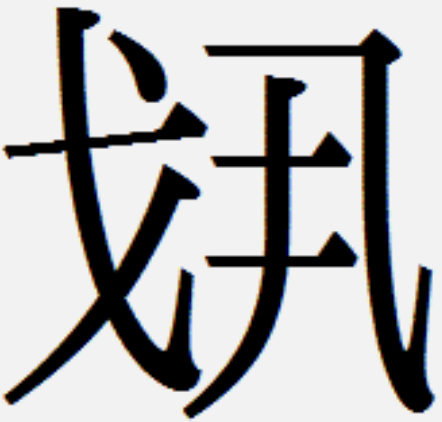
\includegraphics[width=4.5mm]{U+2299A.png}}
%hua4	
%⿰戈丮
{\large{ray{\textsuperscript{·ten}}}},
\textit{ḫwaeX}.	%hwaeX	0007f


\paragraph{\textoversetlarge{19-04}{\huge{咼}}}
{\large{kuay}},
%咼	%wai1	
\textit{kwaeX};	%kwaeX	0018a
騧	%gua1	
{\large{{\textsuperscript{equ·}}kuay}},
\textit{kwae},	%kwae	0018b
%騧	%gua1	
\textit{kwea};	%kwea	0018b
蝸	%wo1	
{\large{{\textsuperscript{serp·}}kuay}},
\textit{kwae},	%kwae	0018c
%蝸	%luo2	
\textit{lwa};	%lwa	0018c
媧	%wa1	
{\large{{\textsuperscript{fem·}}kuay}},
\textit{kwae};	%kwae	0018d
{\large{{\textsuperscript{spirit·}}kuay}},
禍	%huo4	
{\large{kuay}},
\textit{hwaX};	%hwaX	0018f
旤	%huo4	
{\large{kuay{\textsuperscript{·non}}}},
\textit{hwaX}.	%hwaX	0018g
\begin{itemize}[noitemsep]
    \item {\Large{過}}	%guo1	
{\large{{\textsuperscript{amb·}}kuay}}
=
{\large{kuay₂}},
\textit{kwa},	%kwa	0018e
%過	%guo4	
\textit{kwaH};	%kwaH	0018e
薖	%ke1	
{\large{{\textsuperscript{herb:}kuay₂}}},
\textit{khwa}.	%khwa	0018h
\end{itemize}



\paragraph{\textoversetlarge{19-05}{\huge{虧}}}	%kui1	
\textit{khiwe}	%khjwe	0028a

\paragraph{\textoversetlarge{19-06}{\huge{為}}}	%wei2	
{\large{quay}},
\textit{ḫiwe},	%hjwe	0027a
%為	%wei4	
\textit{ḫiweH};	%hjweH	0027a
䦱	%wei3	
{\large{{\textsuperscript{port:}}quay}},
\textit{ḫiweX};	%hjweX	0027f
嬀	%gui1	
{\large{{\textsuperscript{fem·}}quay}},
\textit{kiwe};	%kjwe	0027g
偽	%wei3	
{\large{{\textsuperscript{hom·}}quay}},
\textit{ṅiweH};	%ngjweH	0027k
撝	%hui1	
{\large{{\textsuperscript{man·}}quay}},
\textit{hiwe};	%xjwe	0027l
譌	%e2	
{\large{{\textsuperscript{dic·}}quay}},
\textit{ṅwa}.	%ngwa	0027m




\paragraph{\textoversetlarge{19-07}{\huge{禾}}}
%he2	
{\large{qoy}},
\textit{ḫwa};	%hwa	0008a
和	%he2	
{\large{qoy{\textsuperscript{·or}}}},
\textit{ḫwa},	%hwa	0008e
%和	he4	
\textit{ḫwaH};	%hwaH	0008e
{\large{{\textsuperscript{tibia·}}qoy}},
龢	%he2	
\textit{ḫwa};	%hwa	0008g
盉	%he2	
{\large{qoy{\textsuperscript{:vas}}}},
\textit{ḫwa};	%hwa	0008k
科	%ke1	
{\large{qoy{\textsuperscript{·trull}}}},
\textit{khwa}.	%khwa	0008n

\paragraph{\textoversetlarge{19-08}{\huge{化}}}
%化	%hua4	
{\large{kuay}},
\textit{hwaeH};	%xwaeH	0019a
貨 {\large{kuay{\textsuperscript{:conch}}}},
	%huo4	
\textit{hwaH};	%xwaH	0019c
吪	{\large{{\textsuperscript{or·}}kuay}},
%e2	
\textit{ṅwa};	%ngwa	0019d
訛	%e2	
{\large{{\textsuperscript{dic·}}kuay}},
\textit{ṅwa}.	%ngwa	0019e




\paragraph{\textoversetlarge{19-11}{\huge{臥}}}
%wo4	
\textit{ṅwaH}.	%ngwaH	0009a

\paragraph{\textoversetlarge{19-12}{\huge{危}}}	%wei1	
{\large{koy}},
\textit{ṅiwe};	%ngjwe	0029a
詭	%gui3	
{\large{{\textsuperscript{dic·}}koy}},
\textit{kiweX};	%kjweX	0029b
佹	%gui3	
{\large{{\textsuperscript{hom·}}koy}},
\textit{kiweX};	%kjweX	0029c
垝	%gui3	
{\large{{\textsuperscript{terr·}}koy}},
\textit{kiweX};	%kjweX	0029d
恑	%gui3	
{\large{{\textsuperscript{cor·}}koy}},
\textit{kiweX};	%kjweX	0029e
跪	%gui4	
{\large{{\textsuperscript{ped·}}koy}},
\textit{giweX},	%gjweX	0029f
%跪	%gui4	
\textit{khiweX}.	%khjweX	0029f


\paragraph{\textoversetlarge{19-13}{\huge{瓦}}}
%瓦	%wa3	
\textit{ṅwaeX}.	%ngwaeX	0020a


\paragraph{\textoversetlarge{19-14}{\huge{朵}}}
%duo3	
\textit{twaX};	%twaX	0010a
朶	%duo3	
\textit{twaX}.	%twaX	0010b

\begin{spacing}{0.7}
\paragraph{\textoversetlarge{19-15}{\huge{吹}}}	%chui1	
{\large{th\textoverset{b}{o}y}}
\textit{chiwe},	%tsyhwe	0030a
%吹	%chui4	
\textit{chiweH};	%tsyhweH	0030a
炊	%chui1	
{\large{{\textsuperscript{ign·}}{th\textoverset{b}{o}y}}}
\textit{chiwe}.	%tsyhwe	0030b
\end{spacing}
Baxter and Sagart reconstruct with -r. 


\paragraph{\textoversetlarge{19-16}{\huge{隓}}}
%hui1	
{\large{loy}},
\textit{dwaX};	%dwaX	0011a
\begin{itemize}[noitemsep]
    \item 
{\Large{隋}}	%sui2	
{\large{loy}{\textsuperscript{·carn}}}
= {\large{loy₂}},
\textit{siweH}	%sjweH	0011b
%隋	tuo3	
\textit{thwaX}	%thwaX	0011b
%隋	sui2	
\textit{hiwieH};	%xjwieH	0011b
橢	%tuo3	
{\large{{\textsuperscript{arb·}}loy₂}},
\textit{thwaX};	%thwaX	0011c
嶞	%duo4	
{\large{loy₂{\textsuperscript{:mon}}}},
\textit{dwaX};	%dwaX	0011d
墮	%duo4	
{\large{loy₂{\textsuperscript{:ter}}}},
\textit{dwaX},	%dwaX	0011e
%墮	hui1	
\textit{hiwie};	%xjwie	0011e
隳	%hui1	
{\large{loy₂}{\textsuperscript{:tu}}},
\textit{hiwie};	%xjwie	0011f
隨	%sui2	
{\large{{\textsuperscript{tum·}}loy₂}},
\textit{ziwe};	%zjwe	0011g
髓	%sui3	
{\large{{\textsuperscript{oss·}}loy₂}},
\textit{siweX};	%sjweX	0011h
瀡	%sui3	
{\large{{\textsuperscript{aq·}}loy₂}},
\textit{siweH};	%sjweH	0011i
鬌	%duo3	
{\large{{\textsuperscript{cri:}}loy₂}},
\textit{ḍiwe};	%drjwe	0011j
%鬌	%duo3	
\textit{dwaX},	%dwaX	0011j
%鬌	%duo3	
\textit{twaX};	%twaX	0011j
媠	%duo4	
{\large{{\textsuperscript{fem·}}loy₂}},
\textit{dwaH},	%dwaH	0011k
%媠	%tuo3	
\textit{thwaX};	%thwaX	0011k
惰	%duo4	
{\textsuperscript{cor·}}
{\large{loy₂}},
\textit{dwaH},	%dwaH	0011l
%惰	%duo4	
\textit{dwaX}.	%dwaX	0011l
\end{itemize}

\paragraph{\textoversetlarge{19-17}{\huge{垂}}}	%chui2	
{\large{toy}},
\textit{jiwe};	%dzywe	0031a
陲	%chui2	
{\large{{\textsuperscript{tum·}}toy}},
\textit{jiwe};	%dzywe	0031b
睡	%shui4	
{\large{{\textsuperscript{ocul·}}toy}},
\textit{jiweH};	%dzyweH	0031d
菙	%chui2	
{\large{{\textsuperscript{herb·}}toy}},
\textit{jiweX};	%dzyweX	0031e
甀	%zhui4	
{\large{toy{\textsuperscript{·teg}}}},
\textit{ḍiwe},	%drjwe	0031f
%甀	%zhui4	
\textit{ḍiweH};	%drjweH	0031f
錘	%chui2	
{\large{{\textsuperscript{met·}}toy}},
\textit{ḍiwe},	%drjwe	0031g
%錘	%chui2	
\textit{ḍiweH};	%drjweH	0031g
硾	%zhui4	
{\large{{\textsuperscript{lap·}}toy}},
\textit{ḍiweH};	%drjweH	0031h
捶	%chui2	
{\large{{\textsuperscript{man·}}toy}},
\textit{ciweX};	%tsyweX	0031i
箠	%zhui3	
{\large{{\textsuperscript{bamb:}}toy}},
\textit{ciweX};	%tsyweX	0031j
諈	%zhui4	
{\large{{\textsuperscript{dic·}}toy}},
\textit{ṭiweH};	%trjweH	0031k
埵	%duo3	
{\large{{\textsuperscript{terr·}}toy}},
\textit{twaX};	%twaX	0031l
唾	%tuo4	
{\large{{\textsuperscript{or·}}toy}},
\textit{thwaH}.	%thwaH	0031m


\begin{spacing}{0.7}
\paragraph{\textoversetlarge{19-18}{
\includegraphics[width=9mm]{U+26760.png}}}	
	%luo3	
{\large{r\textoverset{a}{o}y}},
\textit{lwa};	%lwa	%0014a
蠃	%luo3	
{\large{r\textoverset{a}{o}y{\textsuperscript{:serp}}}},
\textit{lwaX};	%lwaX	%0014b
羸	%lei2	
{\large{r\textoverset{a}{o}y{\textsuperscript{:ov}}}},
\textit{liwe};	%ljwe	%0014c
\end{spacing}

Baxter and Sagart reconstruct with -r. 



\paragraph{\textoversetlarge{19-21}{\huge{坐}}}
{\large{tsoy}},
 %zuo4	
\textit{dzwaH},	%dzwaH	0012a
%坐	%zuo4	
\textit{dzwaX};	%dzwaX	0012a
痤	%cuo2	
{\large{{\textsuperscript{infirm·}}tsoy}},
\textit{dzwa};	%dzwa	0012b
挫	%cuo4	
{\large{{\textsuperscript{man·}}tsoy}},
\textit{tswaH};	%tswaH	0012c
剉	%cuo4	
{\large{tsoy{\textsuperscript{·cul}}}},
\textit{tshwaH};	%tshwaH	0012e
脞	%cuo3	
{\large{{\textsuperscript{luna·}}tsoy}},
\textit{tshwaX};	%tshwaX	0012f
髽	%zhua1	
{\large{{\textsuperscript{crin·}}tsoy}},
\textit{tṣwae}.	%tsrwae	0012g
\begin{itemize}[noitemsep]
    \item {\Large{夎}} {\large{tsoy{\textsuperscript{:fem}}}}
    = {\large{tsoy₂}},
蓌	%cuo4	
{\large{{\textsuperscript{herb:}}tsoy₂}},
\textit{tṣaeH},	%tsraeH	0012d
%蓌	%cuo4	
\textit{tswaH}.	%tswaH	0012d
\end{itemize}








\begin{spacing}{0.7}
\paragraph{\textoversetlarge{19-22}{
\includegraphics[width=9mm]{U+27D2A.png}}}	
	%suo3	
{\large{s\textoverset{a}{o}y}},
\textit{swaX};	%swaX	%0013a
瑣	%suo3	
{\large{{\textsuperscript{gem·}}s\textoverset{a}{o}y}},
\textit{swaeX};	%swaeX	%0013b
%瑣	%suo3	
\textit{swaX};	%swaX	%0013b
\end{spacing}

\end{multicols}

\subsection{-a}

\begin{multicols}{2}

\begin{spacing}{0.7} 
\paragraph{\textoversetlarge{01-01}{\huge{古}}}	
%古	%gu3	
{\large{ka}},
\textit{kuX};	%kuX	0049a
姑	%gu1	
{\large{{\textsuperscript{fem·}}ka}},
\textit{ku};	%ku	0049g
沽	%gu1	
{\large{{\textsuperscript{aq·}}ka}},
\textit{ku};	%ku	0049k
罟	%gu3	
{\large{{\textsuperscript{nass:}}ka}},
\textit{kuX};	%kuX	0049m
蛄	%gu1	
{\large{{\textsuperscript{serp·}}ka}},
\textit{ku};	%ku	0049o
盬	%gu3	
{\large{{\textsuperscript{observ·}}ka}}
\textit{kuX};	%kuX	0049q
䀇 \footnote{SWJZ: 从皿从缶，古聲。, but I have my doubts.}	%gu3	
\textit{kuX};	%kuX	0049r
枯	%ku1	
{\large{{\textsuperscript{arb·}}ka}},
\textit{khu};	%khu	0049t
岵	%hu4	
{\large{{\textsuperscript{mon·}}ka}},
\textit{huX};	%huX	0049v
怙	%hu4	
{\large{{\textsuperscript{cor·}}ka}},
\textit{huX};	%huX	0049x
祜	%hu4	
{\large{{\textsuperscript{spirit·}}ka}},
\textit{huX};	%huX	0049y
酤	%gu1	
{\large{{\textsuperscript{vin·}}ka}},
\textit{ḫuX};	%huX	0049b'
故	%gu4	
{\large{ka{\textsuperscript{·fer}}}},
\textit{kuH};	%kuH	0049i
\begin{itemize}[noitemsep]
    \item {\Large{固}}	%gu4	
{\large{{\textsuperscript{cla:}}ka}}
= {\large{k\textoverset{a}{a}}},
\textit{kuH};	%kuH	0049f
錮	%gu4	
{\large{{\textsuperscript{met·}}k\textoverset{a}{a}}},
\textit{kuH};	%kuH	0049e'
箇	%ge4	
{\large{{\textsuperscript{bamb:}}k\textoverset{a}{a}}},
\textit{kaH};	%kaH	0049f'
\item {\Large{胡}}	%hu2	
{\large{ka{\textsuperscript{·carn}}}} = {\large{g\textoverset{a}{a}}},
\textit{ḫu};	%hu	0049a'
瑚	%hu2	
{\large{{\textsuperscript{gem·}}g\textoverset{a}{a}}},
\textit{ḫu};	%hu	0049i'
湖	%hu2	
{\large{{\textsuperscript{aq·}}g\textoverset{a}{a}}},
\textit{ḫu};	%hu	0049j'
葫	%hu2	
{\large{{\textsuperscript{herb:}}g\textoverset{a}{a}}},
\textit{ḫu};	%hu	0049k'
餬	%hu2	
{\large{{\textsuperscript{ed·}}g\textoverset{a}{a}}},
\textit{ḫu};	%hu	0049l'
鶘	%hu2	
{\large{g\textoverset{a}{a}{\textsuperscript{·av}}}},
\textit{ḫu};	%hu	0049m'
    \item  {\Large{居}}	%ju1	
{\large{{\textsuperscript{cadaver·}}ka}}
= 
{\large{k\textoverset{b}{a}}},
\textit{kiə},	%kjo	0049c'
%居	%ju1	
\textit{kiəH};	%kjoH	0049c'
倨	%ju4	
{\large{{\textsuperscript{hom·}}k\textoverset{b}{a}}},
\textit{kiəH};	%kjoH	0049n'
据	%ju1	
{\large{{\textsuperscript{man·}}k\textoverset{b}{a}}},
\textit{kiə};	%kjo	0049o'
琚	%ju1	
{\large{{\textsuperscript{gem·}}k\textoverset{b}{a}}},
\textit{kiə};	%kjo	0049p'
裾	%ju1	
{\large{{\textsuperscript{vest·}}k\textoverset{b}{a}}},
\textit{kiə};	%kjo	0049q'
踞	%ju4	
{\large{{\textsuperscript{ped·}}k\textoverset{b}{a}}},
\textit{kiəH};	%kjoH	0049r'
鋸	%ju4	
{\large{{\textsuperscript{met·}}k\textoverset{b}{a}}},
\textit{kiəH};	%kjoH	0049s'
椐	%ju1	
{\large{{\textsuperscript{arb·}}k\textoverset{b}{a}}},
\textit{khiə},	%khjo	0049t'
%椐	%ju1	
\textit{kiəH};	%kjoH	0049t'
腒	%ju1	
{\large{{\textsuperscript{carn·}}k\textoverset{b}{a}}},
\textit{giə},	%gjo	0049u'
%腒	%ju1	
\textit{kiə};	%kjo	0049u'
\item {\Large{辜}}	%gu1	
{\large{ka{\textsuperscript{:acr}}}}
= {\large{k\textoverset{a}{a}₂}},
\textit{ku};	%ku	0049p
橭	%gu1	
{\large{{\textsuperscript{arb·}}k\textoverset{a}{a}₂}},
\textit{khu},	%khu	0049g'
%橭	%gu1	
\textit{ku};	%ku	0049g'
\item {\Large{苦}}	%ku3	
{\large{{\textsuperscript{herb·}}ka}} = {\large{k\textoverset{a}{a}₃}},
\textit{khuX},	%khuX	0049u %苦	%gu3	
\textit{kuX};	%kuX	0049u
楛	%hu4	
{\large{{\textsuperscript{arb·}}k\textoverset{a}{a}₃}},
\textit{ḫuX}.	%huX	0049h'
\end{itemize}
\end{spacing}



\begin{spacing}{0.7} 
\paragraph{\textoversetlarge{01-02}{\huge{鼓}}}	
{\large{k\textoverset{a}{a}}},
%鼓	%gu3	
\textit{kuX};	%kuX	0050a
鼔	%gu3	
\textit{kuX};	%kuX	0050b
瞽	%gu3
{\large{k\textoverset{a}{a}}{\textsuperscript{:ocul}}},
\textit{kuX};	%kuX	0050g
\end{spacing}




\paragraph{\textoversetlarge{01-03}{\huge{股}}}	
%股	%gu3	
\textit{kuX};	%kuX	0051a
羖	%gu3	
\textit{kuX};	%kuX	0051b
\paragraph{\textoversetlarge{01-04}{\huge{蠱}}}	
%蠱	%gu3	
\textit{kuX};	%kuX	0052a

\paragraph{\textoversetlarge{01-05}{\huge{壺}}}	
%壺	%hu2	
\textit{ḫu};	%hu	0056a

\begin{spacing}{0.7} 
\paragraph{\textoversetlarge{01-06}{\huge{戶}}}	
{\large{ka}},
%戶	%hu4	
\textit{ḫuX};	%huX	0053a
扈	%hu4	
{\large{ka{\textsuperscript{·urb}}}},
\textit{ḫuX};	%huX	0053c
鳸	%hu4	
{\large{ka{\textsuperscript{·av}}}},
\textit{ḫuX};	%huX	0053e
\begin{itemize}[noitemsep]
    \item {\Large{雇}}	%gu4	
{\large{ka{\textsuperscript{·passer}}}} = {\large{ka₂}},
\textit{kuH};	%kuH	0053d
顧	%gu4	
{\large{ka₂{\textsuperscript{·fac}}}}, 
\textit{kuH};	%kuH	0053g
\end{itemize}
\end{spacing}

\begin{spacing}{0.7} 
\paragraph{\textoversetlarge{01-07}{\huge{互}}}	
%互	%hu4	
{\large{g\textoverset{a}{a}}},
\textit{ḫuH};	%huH	0054a
枑	%hu4	
{\large{{\textsuperscript{arb·}}g\textoverset{a}{a}}},
\textit{ḫuH};	%huH	0054b
沍	%hu4	
{\large{{\textsuperscript{aq·}}g\textoverset{a}{a}}},
\textit{ḫuH}.	%huH	0054c
\end{spacing}


\paragraph{\textoversetlarge{01-10}{\huge{車}}}	
%車	%ju1	
\textit{kiə},	%kjo	0074a
%車	%che1	
\textit{chiae};	%tsyhae	0074a
庫	%ku4	
\textit{khuH};	%khuH	0074e





\begin{spacing}{0.7}
\paragraph{\textoversetlarge{01-11}{\huge{家}}}	%jia1	
{\large{kr\textoverset{a}{a}}},
\textit{kae};	%kae	0032a
嫁	%jia4	
{\large{{\textsuperscript{fem·}}kr\textoverset{a}{a}}},
\textit{kaeH};	%kaeH	0032e
稼	%jia4	
{\large{{\textsuperscript{gran·}}kr\textoverset{a}{a}}},
\textit{kaeH}.	%kaeH	0032f
\end{spacing}

\begin{spacing}{0.7}
\paragraph{\textoversetlarge{01-12}{\huge{叚}}}		
%叚	%jia3	
{\large{kr\textoverset{a}{a}}},
\textit{kaeX};	%kaeX	0033a
假	%jia3	
{\large{{\textsuperscript{hom·}}kr\textoverset{a}{a}}},
\textit{kaeX};	%kaeX	0033c
嘏	%jia3	
{\large{{\textsuperscript{antiqu·}}kr\textoverset{a}{a}}},
\textit{kaeX};	%kaeX	0033d
葭	%jia1	
{\large{{\textsuperscript{herb:}}kr\textoverset{a}{a}}},
\textit{kae};	%kae	0033e
豭	%jia1	
{\large{{\textsuperscript{porc·}}kr\textoverset{a}{a}}},
\textit{kae};	%kae	0033f
暇	%xia4	
{\large{{\textsuperscript{sol·}}kr\textoverset{a}{a}}},
\textit{ḫaeH};	%haeH	0033g
瑕	%xia2	
{\large{{\textsuperscript{gem·}}kr\textoverset{a}{a}}},
\textit{ḫae};	%hae	0033h
蝦	%ha2	
{\large{{\textsuperscript{serp·}}kr\textoverset{a}{a}}},
\textit{ḫae};	%hae	0033i
遐	%xia2	
{\large{{\textsuperscript{amb·}}kr\textoverset{a}{a}}},
\textit{ḫae};	%hae	0033j
霞	%xia2	
{\large{{\textsuperscript{pluv:}}kr\textoverset{a}{a}}},
\textit{ḫae};	%hae	0033k
騢	%xia2	
{\large{{\textsuperscript{equ·}}kr\textoverset{a}{a}}},
\textit{ḫae}.	%hae	0033l
\end{spacing}





\paragraph{\textoversetlarge{01-13}{\huge{斝}}}	%jia3	
\textit{kaeX}	%kaeX	0034a

\paragraph{\textoversetlarge{01-14}{\huge{下}}}	%xia4	
\textit{ḫaeH},	%haeH	0035a
%下	xia4	
\textit{ḫaeX};	%haeX	0035a
芐	%xia4	
\textit{ḫaeH},	%haeH	0035d
%芐	hu4	
\textit{ḫuX}.	%huX	0035d

\paragraph{\textoversetlarge{01-15}{\huge{夏}}}	
%夏	%xia4	
\textit{ḫaeH},	%haeH	0036a
%夏	%xia4	
\textit{ḫaeX};	%haeX	0036a
廈	%xia4	
\textit{ḫaeX};	%haeX	0036c
厦	%xia4	
\textit{ḫaeX}.	%haeX	0036d


\paragraph{\textoversetlarge{01-16}{\huge{襾}}}	
%襾	%ya4	
{\large{qa}},
\textit{haeX};	%xaeX	0038a
\begin{itemize}
    \item 
{\Large{賈}}	%jia4	
{\large{qa{\textsuperscript{·conch}}}} = {\large{ka}},
\textit{kaeH},	%kaeH	0038b
%賈	%gu3	
\textit{kuX};	%kuX	0038b
價	%jia4	
\textit{kaeH};	%kaeH	0038c
檟	%jia3	
\textit{kaeX};	%kaeX	0038d
\end{itemize}

\begin{spacing}{0.7} 
\paragraph{\textoversetlarge{01-17}{\huge{乎}}}	
{\large{q\textoverset{a}{a}}},
%乎	%hu1	
\textit{ḫu};	%hu	0055a
呼	%hu1	
{\large{{\textsuperscript{or·}}q\textoverset{a}{a}}},
\textit{hu},	%xu	0055h
%呼	%hù	
\textit{huH};	%xuH	0055h
\begin{itemize}[noitemsep]
    \item {\Large{虖}}	%hu2	
{\large{{\textsuperscript{tigr·}}q\textoverset{a}{a}}} = {\large{q\textoverset{a}{a}₂}},
\textit{ḫu};	%hu	0055e
嘑	%hu1	
{\large{{\textsuperscript{or·}}q\textoverset{a}{a}₂}},
\textit{hu}.	%xu	0055i
\end{itemize}
\end{spacing}


\paragraph{\textoversetlarge{01-18}{\huge{虍}}}	
%虍	%hu1	
\textit{hu};	%xu	0057a
虎	%hu3	
\textit{huX};	%xuX	0057b
琥	%hu3	
\textit{huX};	%xuX	0057f



\paragraph{\textoversetlarge{01-18}{
\includegraphics[width=8mm]{U+271A8.png}}}	
{\large{ra}},
 %lu2	
\textit{lu};	%lu	0069a
虜	%lu3	
{\large{ra\textsuperscript{·masc}}},
\textit{luX};	%luX	0069e
膚	%fu1	
{\large{ra\textsuperscript{·ventri}}},
\textit{piu};	%pju	0069g
\begin{itemize}[noitemsep]
    \item {\Large{慮}}	%lü4	
{\large{ra\textsuperscript{·cogit}}} = {\large{ra₂}},
\textit{liəH};	%ljoH	0069f
藘	%lü2	
{\large{\textsuperscript{herb·}ra₂}}, 
\textit{liə};	%ljo	0069u
鑢	%lü4	
{\large{\textsuperscript{met·}ra₂}}, 
\textit{liəH};	%ljoH	0069v
攄	%shu1
{\large{\textsuperscript{man·}ra₂}}, 
\textit{ṭhiə};	%trhjo	0069x
\item {\Large{盧}}	%lu2	
{\large{ra\textsuperscript{:vas}}},
\textit{lu};	%lu	0069d
壚	%lu2	
{\large{\textsuperscript{terr·}ra₃}}, 
\textit{lu};	%lu	0069j
櫨	%lu2	
{\large{\textsuperscript{arb·}ra₃}}, 
\textit{lu};	%lu	0069k
爐	%lu2	
{\large{\textsuperscript{ign·}ra₃}}, 
\textit{lu};	%lu	0069l
鑪	%lu2	
{\large{\textsuperscript{met·}ra₃}}, 
\textit{lu};	%lu	0069m
籚	%lu2	
{\large{\textsuperscript{bamb·}ra₃}}, 
\textit{lu};	%lu	0069n
纑	%lu2	
{\large{\textsuperscript{ser·}ra₃}}, 
\textit{lu};	%lu	0069o
顱	%lu2	
{\large{ra₃\textsuperscript{·fac}}}, 
\textit{lu};	%lu	0069p
廬	%lu2	
{\large{\textsuperscript{lax·}ra₃}}, 
\textit{liə};	%ljo	0069q
臚	%lu2	
{\large{\textsuperscript{carn·}ra₃}}, 
\textit{liə};	%ljo	0069r
儢	%lü3	
{\large{\textsuperscript{hom·}ra₃}}, 
\textit{liəX}.	%ljoX	0069t
\end{itemize}


\begin{spacing}{0.7} 
\paragraph{\textoversetlarge{01-18}{\huge{虛}}}	
 {\large{q\textoverset{b}{a}}},  
%虛	%xu1	
\textit{khiə},	%khjo	0078a
%虛	%xu1	
\textit{hiə};	%xjo	0078a
墟	%xu1	
{\large{\textsuperscript{terr·}q\textoverset{b}{a}}},  
\textit{khiə};	%khjo	0078b
歔	%xu1	
{\large{q\textoverset{b}{a}\textsuperscript{·dehab}}},  
\textit{hiə},	%xjo	0078c
%歔	%xu1	
\textit{hiəH};	%xjoH	0078c
噓	%xu1	
{\large{\textsuperscript{or·}q\textoverset{b}{a}}},  
\textit{hiə},	%xjo	0078d
%噓	%xu4	
\textit{hiəH};	%xjoH	0078d
虡\footnote{I need to look into this character more.}	%ju4	
\textit{giəX};	%gjoX	0078e
	%ju4	
{
\includegraphics[width=4.5mm]{U+25CA4.png}}
{\large{\textsuperscript{bamb·}q\textoverset{b}{a}}},  
\textit{giəX}.	%gjoX	0078g
\end{spacing}

\paragraph{\textoversetlarge{01-18}{\huge{處}}}	
%處	%chu4	
\textit{chiəH},	%tsyhoH	0085a
%處	%chu3	
\textit{chiəX};	%tsyhoX	0085a




\begin{spacing}{0.7} 
\paragraph{\textoversetlarge{01-19}{\huge{巨}}}	
{\large{k\textoverset{b}{a}}}, 
%巨	%ju4	
\textit{giəX},	%gjoX	0095a
%巨	%ju4	
\textit{kiuX};	%kjuX	0095a
柜	%ju3	
\textit{kiuX};	%kjuX	0095f
蚷	%qu2	
\textit{giə};	%gjo	0095h
拒	%ju4	
\textit{giəX},	%gjoX	0095i
%拒	%ju3	
\textit{kiuX};	%kjuX	0095i
秬	%ju4	
\textit{giəX};	%gjoX	0095j
粔	%ju4	
\textit{giəX};	%gjoX	0095n
耟	%ju4	
\textit{giəX};	%gjoX	0095o
詎	%ju4	
\textit{giəH},	%gjoH	0095p
%詎	%ju4	
\textit{giəX};	%gjoX	0095p
距	%ju4	
\textit{giəX};	%gjoX	0095q
鉅	%ju4	
\textit{giəX};	%gjoX	0095r
\begin{itemize}[noitemsep]
    \item {\Large{矩}}	%ju3	
\textit{kiuX};	%kjuX	0095c
榘	%ju3	
\textit{kiuX};	%kjuX	0095e
%��	%koi4	
{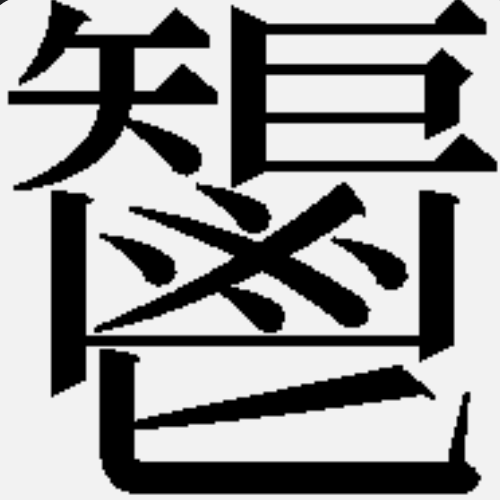
\includegraphics[width=4mm]{U+29C24.png}}
%⿱矩鬯
\textit{giuX};	%gjuX	0095k
\item {\Large{洰}} \textit{giuX};
%臼 giuwX + 許 xuX = giuX
渠	%qu2	
\textit{giə};	%gjo	0095g
\end{itemize}
\end{spacing}

I do not see how ka and kua can mix in one XS series. 






\begin{spacing}{0.7}
\paragraph{\textoversetlarge{01-21}{\huge{瓜}}}	
%瓜	%gua1	
{\large{ku\textoverset{a}{a}}},
\textit{kwae};	%kwae	0041a
呱	%gu1	
{\large{{\textsuperscript{or·}}ku\textoverset{a}{a}}},
\textit{ku};	%ku	0041b
孤	%gu1	
{\large{{\textsuperscript{fili·}}ku\textoverset{a}{a}}},
\textit{ku};	%ku	0041c
罛	%gu1	
{\large{{\textsuperscript{nass:}}ku\textoverset{a}{a}}},
\textit{ku};	%ku	0041d
苽	%gu1	
{\large{{\textsuperscript{herb·}}ku\textoverset{a}{a}}},
\textit{ku};	%ku	0041e
觚	%gu1	
{\large{{\textsuperscript{corn·}}ku\textoverset{a}{a}}},
\textit{ku};	%ku	0041f
軱	%gu1	
{\large{{\textsuperscript{vehic·}}ku\textoverset{a}{a}}},
\textit{ku};	%ku	0041g
弧
{\large{{\textsuperscript{arc·}}ku\textoverset{a}{a}}},
	%hu2	
\textit{hu};	%hu	0041h
狐	%hu2	
{\large{{\textsuperscript{can·}}ku\textoverset{a}{a}}},
\textit{hu};	%hu	0041i
\end{spacing}



\paragraph{\textoversetlarge{01-22}{\huge{寡}}}	
%寡	%gua3	
\textit{kwaeX};	%kwaeX	0042a

\paragraph{\textoversetlarge{01-22}{\huge{夸}}}	
%夸	%kua1	
{\large{qua}},
\textit{khwae};	%khwae	0043a
誇	%kua1	
{\large{{\textsuperscript{dic·}}    qua}}, 
\textit{khwae};	%khwae	0043b
姱	%kua1	
{\large{{\textsuperscript{fem·}}    qua}}, 
\textit{khwae};	%khwae	0043c
跨	%ku4	
{\large{{\textsuperscript{ped·}}    qua}}, 
\textit{khuH},	%khuH	0043d
%跨	%kua4	
\textit{khwaeH};	%khwaeH	0043d
荂	%kua1	
{\large{{\textsuperscript{herb:}}    qua}}, 
\textit{khwae},	%khwae	0043e
%荂	%kua1	
\textit{hiu};	%xju	0043e
刳	%ku1	
{\large{qua{\textsuperscript{:cul}}}}, 
\textit{khuH};	%khuH	0043f
挎	%ku1	
{\large{{\textsuperscript{man·}}qua}}, 
\textit{khu};	%khu	0043g
袴	%ku4	
{\large{{\textsuperscript{vest·}}qua}},
\textit{khuH};	%khuH	0043h
絝	%ku4	
{\large{{\textsuperscript{ser·}}qua}},
\textit{khuH};	%khuH	0043i
\begin{itemize}[noitemsep]
    \item 瓠	%hu2	
{\large{qua{\textsuperscript{·瓜}}}},
\textit{ḫu} = {\large{ɢua}},	%hu	0043j
%瓠	%hu4	
\textit{ḫuH};	%huH	0043j
槬	%hua4	
{\large{{\textsuperscript{arb·}}ɢua}},
\textit{ḫwaeH};	%hwaeH	0043l
摦	%hua4	
{\large{{\textsuperscript{man·}}ɢua}},
\textit{ḫwaeH};	%hwaeH	0043m
\end{itemize}

洿	%wu1	
{\large{{\textsuperscript{aq·}}qua}},
\textit{{\sil{ꞏ}}u};	%'u	0043k


\paragraph{\textoversetlarge{01-23}{\huge{于}}}	
%于	%yu2	
\textit{ḫiu};	%hju	0097a
杇	%wu1	
\textit{{\sil{ꞏ}}u};	%'u	0097a'
汙	%wa1	
\textit{{\sil{ꞏ}}wae};	%'wae	0097b'
污	%wu1	
\textit{{\sil{ꞏ}}u};	%'u	0097c'
污	%wa1	
\textit{{\sil{ꞏ}}wae};	%'wae	0097c'
冔	%xu3	
\textit{hiuX};	%xjuX	0097d'
宇	%yu3	
\textit{ḫiuX};	%hjuX	0097h
杅	%yu2
\textit{ḫiu};	%hju	0097i
玗	%yu2	
\textit{ḫiu};	%hju	0097j
盂	%yu2	
\textit{ḫiu};	%hju	0097k
竽	%yu2	
\textit{ḫiu};	%hju	0097n
芋	%yu4	
\textit{ḫiuH};	%hjuH	0097o
迂	%yu1	
\textit{{\sil{ꞏ}}iu};	%'ju	0097p
迂	%yu1	
\textit{ḫiu};	%hju	0097p
雩	%yu2	
\textit{ḫiu};	%hju	0097q
吁	%xu1	
\textit{hiu};	%xju	0097t
盱	%xu1	
\textit{hiu};	%xju	0097u
訏	%xu1	
\textit{hiu};	%xju	0097v
紆	%yu1	
\textit{{\sil{ꞏ}}iu};	%'ju	0097y
圩	%wu1	
\textit{{\sil{ꞏ}}u};	%'u	0097z

\paragraph{\textoversetlarge{01-24}{\huge{羽}}}	
%羽	%yu3	
\textit{ḫiuX};	%hjuX	0098a
栩	%xu3	
\textit{hiuX};	%xjuX	0098c
詡	%xu3	
\textit{hiuX};	%xjuX	0098d

\paragraph{\textoversetlarge{01-25}{\huge{禹}}}	
%禹	%yu3	
\textit{ḫiuX};	%hjuX	0099a
偊	%yu3	
\textit{ḫiuX};	%hjuX	0099d
楀	%ju3	
\textit{kiuX};	%kjuX	0099e
萭	%ki3	
\textit{kiuX};	%kjuX	0099f
踽	%ju3	
\textit{kiuX};	%kjuX	0099g

\paragraph{\textoversetlarge{01-26}{\huge{雨}}}	
%雨	%yu4	
\textit{ḫiuH},	%hjuH	0100a
%雨	%yu3	
\textit{ḫiuX};	%hjuX	0100a





\begin{spacing}{0.7}
\paragraph{\textoversetlarge{01-27}{\huge{華}}}	
{\large{qur\textoverset{a}{a}}},
%華	%hua2	
\textit{ḫwae},	%hwae	0044a
%華	%hua4	
\textit{ḫwaeH},	%hwaeH	0044a
%華	%hua1	
\textit{hwae};	%xwae	0044a
驊	%hua2	
{\large{{\textsuperscript{equ·}}qur\textoverset{a}{a}}},
\textit{ḫwae};	%hwae	0044c
譁	%hua2	
{\large{{\textsuperscript{dic·}}qur\textoverset{a}{a}}},
\textit{hwae}.	%xwae	0044d
\end{spacing}


\paragraph{\textoversetlarge{01-28}{\huge{烏}}}	
%烏	%wu1	
{\large{a}},
\textit{{\sil{ꞏ}}u};	%'u	0061a
嗚	%wu1	
{\large{{\textsuperscript{or·}}a}},
\textit{{\sil{ꞏ}}u};	%'u	0061d
\begin{itemize}[noitemsep]
    \item {\Large{於}}\footnote{I will have to look into this character more.}	%yu2	
\textit{{\sil{ꞏ}}iə},	%'jo	0061e
%於	%yu4?	
\textit{{\sil{ꞏ}}iəH},	%'joH	0061e
%於	%wu1	
\textit{{\sil{ꞏ}}u};	%'u	0061e
棜	%yu4	
{\large{{\textsuperscript{arb·}}a}},
\textit{{\sil{ꞏ}}iəH};	%'joH	0061g
瘀	%yu1	
{\large{{\textsuperscript{infirm·}}a}},
\textit{{\sil{ꞏ}}iəH};	%'joH	0061h
菸	%yu1	
{\large{{\textsuperscript{herb·}}a}},
\textit{{\sil{ꞏ}}iə};	%'jo	0061i
\end{itemize}


\paragraph{\textoversetlarge{01-29}{\huge{五}}}	
%五	%wu3	
{\large{ṅa}},
\textit{ṅuX};	%nguX	0058a
伍	%wu3	
{\large{{\textsuperscript{hom·}}ṅa}},
\textit{ṅuX};	%nguX	0058e
\begin{itemize}[noitemsep]
    \item {\Large{吾}}	%wu2	
{\large{ṅa{\textsuperscript{:or}}}} = {\large{ṅa₂}},
\textit{ṅu};	%ngu	0058f
悟	%wu4	
{\large{{\textsuperscript{cor·}}ṅa₂}}, 
\textit{ṅuH};	%nguH	0058j
捂	%wu3	
{\large{{\textsuperscript{man·}}ṅa₂}}, 
\textit{ṅuH};	%nguH	0058k
晤	%wu4	
{\large{{\textsuperscript{sol·}}ṅa₂}}, 
\textit{ṅuH};	%nguH	0058l
梧	%wu2	
{\large{{\textsuperscript{arb·}}ṅa₂}}, 
\textit{ṅu};	%ngu	0058m
寤	%wu4	
{\large{{\textsuperscript{somn·}}ṅa₂}}, 
\textit{ṅuH};	%nguH	0058n
啎	%wu4	
{\large{{\textsuperscript{meridi·}}ṅa₂}}, 
\textit{ṅuH};	%nguH	0058o
圄	%yu3	
{\large{{\textsuperscript{cla:}}ṅa₂}}, 
\textit{ṅiəX};	%ngjoX	0058p
敔	%yu3	
{\large{ṅa₂{\textsuperscript{·fer}}}}, 
\textit{ṅiəX};	%ngjoX	0058q
衙	%ya2	
{\large{{\textsuperscript{eo·}}ṅa₂}}, 
\textit{ṅae},	%ngae	0058s
%衙	%yu2	
\textit{ṅiə};	%ngjo	0058s
語	%yu4	
{\large{{\textsuperscript{dic·}}ṅa₂}}, 
\textit{ṅiəH},	%ngjoH	0058t
%語	%yu3	
\textit{ṅiəX};	%ngjoX	0058t
鋙	%yu2	
{\large{{\textsuperscript{met·}}ṅa₂}}, 
\textit{ṅiə},	%ngjo	0058v
%鋙	%yu3	
\textit{ṅiəX}.	%ngjoX	0058v
\end{itemize}



\begin{spacing}{0.7} 
\paragraph{\textoversetlarge{01-30}{\huge{午}}}	
{\large{ṅa}},
%午	%wu3	
\textit{ṅuX};	%nguX	0060a
仵	%wu3	
{{\textsuperscript{hom·}}\large{ṅa}},
\textit{ṅuH},	%nguH	0060f
%仵	%wu3	
\textit{ṅuX};	%nguX	0060f
忤	%wu4	
{{\textsuperscript{cor·}}\large{ṅa}},
\textit{ṅuH};	%nguH	0060g
迕	%wu4	
{{\textsuperscript{amb·}}\large{ṅa}},
\textit{ṅuH};	%nguH	0060h
杵
%杵	%chu3	
{{\textsuperscript{arb·}}\large{ṅa}},
\textit{chiəX};	%tsyhoX	0086a
\begin{itemize}[noitemsep]
    \item {\Large{許}}	%xu3	
{\large{\textsuperscript{dic·}ṅa}} = {\large{ṅha}},
\textit{hiəX},	%xjoX	0060i
%許	%hu3	
\textit{huX};	%xuX	0060i
滸	%hu3	
{{\textsuperscript{aq·}}\large{ṅha}},
\textit{huX};	%xuX	0060k
\item {\Large{御}}	%yu4	
{\large{ṅa}} = {\large{ṅ\textoverset{b}{a}}},
\textit{ṅiəH};	%ngjoH	0060l
禦	%yu4	
 {\large{ṅ\textoverset{b}{a}{\textsuperscript{:spir}}}}, 
\textit{ṅiəX}.	%ngjoX	0060p
\end{itemize}
\end{spacing}

\begin{spacing}{0.7} 
\paragraph{\textoversetlarge{01-31}{\huge{魚}}}	
{\large{ṅa}},
%魚	%yu2	
\textit{ṅiə};	%ngjo	0079a
漁	%yu2	
{\large{\textsuperscript{aq·}ṅa}},
\textit{ṅiə};	%ngjo	0079g
䱷\footnote{I need to look into this character more.}	%yu2	
\textit{ṅiə};	%ngjo	0079m
%\paragraph{\textoversetlarge{01-31}
\begin{itemize}[noitemsep]
    \item {\Large{穌}}
{\large{ṅa\textsuperscript{·gran}}} = {\large{sa}},
%穌	%su1	
\textit{su};	%su	0067a
蘇	%su1	
{\large{\textsuperscript{herb·}sa}},
\textit{su}.	%su	0067c
\end{itemize}
\end{spacing}

\paragraph{\textoversetlarge{01-32}{\huge{圉}}}	
%圉	%yu3	
\textit{ṅiəH},	%ngjoH	0081a
%圉	%yu3	
\textit{ṅiəX};	%ngjoX	0081a



\paragraph{\textoversetlarge{01-33}{\huge{馭}}}	
%馭	%yu4	
\textit{ṅiəH};	%ngjoH	0080a





\begin{spacing}{0.7}
\paragraph{\textoversetlarge{01-34}{\huge{牙}}}	
%牙	%ya2	
{\large{qr\textoverset{a}{a}}},
\textit{ṅae};	%ngae	0037a
庌	%ya3	
{\large{{\textsuperscript{lax·}}qr\textoverset{a}{a}}},
\textit{ṅaeX};	%ngaeX	0037c
芽	%ya2	
{\large{{\textsuperscript{herb·}}qr\textoverset{a}{a}}},
\textit{ṅae};	%ngae	0037d
訝	%ya4	
{\large{{\textsuperscript{dic·}}qr\textoverset{a}{a}}},
\textit{ṅaeH};	%ngaeH	0037e
迓	%ya4	
{\large{{\textsuperscript{amb·}}qr\textoverset{a}{a}}},
\textit{ṅaeH};	%ngaeH	0037f
雅	%ya3	
{\large{qr\textoverset{a}{a}{\textsuperscript{·passer}}}},
\textit{ṅaeX};	%ngaeX	0037g
鴉	%ya1	
{\large{qr\textoverset{a}{a}{\textsuperscript{·av}}}},
\textit{{\sil{ꞏ}}ae};	%'ae	0037h
\begin{itemize}
    \item {\Large{邪}}
%邪	%ya2	
\textit{yae},	%yae	0047a
%邪	%xie2	
\textit{ziae},	%zjae	0047a
%邪	%xu2	
\textit{ziə};	%zjo	0047a
耶	%ye2	
{\large{{\textsuperscript{aur·}}xxx}},
\textit{yiae};	%yae	0047b
衺	%xie2	
{\large{{\textsuperscript{vest:}}qra}}, 
%从衣牙声
\textit{ziae}.\footnote{I need to look into why this character is put in GSR 0047 and not GSR 0037.}	%zjae	0047c
\end{itemize}
\end{spacing}


   


\paragraph{\textoversetlarge{01-34}{\huge{舉}}}	
%舉	%ju3	
\textit{kiəX};	%kjoX	0075a

\paragraph{\textoversetlarge{01-35}{\huge{吳}}}	
%吳	%wu2	
{\large{ṅa}},
\textit{ṅu};	%ngu	0059a
誤	%wu4	
{\large{{\textsuperscript{dic·}}ṅa}}, 
\textit{ṅuH};	%nguH	0059d
悞	%wu4	
{\large{{\textsuperscript{cor·}}ṅa}}, 
\textit{ṅuH};	%nguH	0059e
俁	%yu3	
{\large{{\textsuperscript{hom·}}ṅa}}, 
\textit{ṅiuX};	%ngjuX	0059f
娛	%yu2	
{\large{{\textsuperscript{fem·}}ṅa}}, 
\textit{ṅiu};	%ngju	0059g
麌	%yu3	
{\large{{\textsuperscript{cerv·}}ṅa}}, 
\textit{ṅiuX};	%ngjuX	0059j

\begin{itemize}[noitemsep]
    \item {\Large{虞}}	%yu2	
{\large{{\textsuperscript{tigr·}}ṅa}}
= {\large{ṅa₂}}, 
\textit{ṅiu};	%ngju	0059h
噳	%yu3	
{\large{{\textsuperscript{or·}}ṅa₂}}, 
\textit{ṅiuX}.	%ngjuX	0059k
\end{itemize}


\paragraph{\textoversetlarge{01-36}{\huge{土}}}	
%土	%tu3	
{\large{ta}},
\textit{duX},	%duX	0062a
%土	%tu3	
\textit{thuX};	%thuX	0062a
吐	%tu4	
{\large{\textsuperscript{or·}ta}},
\textit{thuH},	
%thuH	0062d
%吐	%tu3	
\textit{thuX};
%thuX	0062d
徒	%tu2	
{\large{\textsuperscript{amb·}ta}},
\textit{du};	%du	0062e
杜	%du4	
{\large{\textsuperscript{arb·}ta}},
\textit{duX},	%duX	0062g
%社	%she4
\textit{jiaeX};	%dzyaeX	0062j

\paragraph{\textoversetlarge{01-37}{\huge{圖}}}	
%圖	%tu2	
\textit{du};	%du	0064a


\begin{spacing}{0.7}
\paragraph{\textoversetlarge{01-38}{\huge{者}}}	
%者	%zhe3	
{\large{ta}}, 
\textit{ciaeX};	%tsyaeX	0045a
赭	%zhe3	
{\large{{\textsuperscript{ruf·}}ta}},
\textit{ciaeX};	%tsyaeX	0045d
奢	%she1	
{\large{{\textsuperscript{magn:}}ta}}, 
\textit{śiae};	%syae	0045e
褚	%zhu3	
{\large{{\textsuperscript{vest·}}ta}},
\textit{ṭiəX};	%trjoX	0045g
帾	%du3	
{\large{{\textsuperscript{lint·}}ta}},
\textit{tuX};	%tuX	0045b'
睹	%du3	
{\large{{\textsuperscript{ocul·}}ta}},
\textit{tuX};	%tuX	0045c'
覩	%du3	
{\large{ta{\textsuperscript{·vid}}}},
\textit{tuX};	%tuX	0045d'
都	%du1	
{\large{ta{\textsuperscript{·urb}}}},
\textit{tu};	%tu	0045e'
楮	%chu3	
{\large{{\textsuperscript{arb·}}ta}},
\textit{ṭhiəX},	%trhjoX	0045i
%楮	%chu3	
\textit{tuX};	%tuX	0045i
屠	%tu2	
{\large{{\textsuperscript{ost·}}ta}},
\textit{du};	%du	0045i'
箸	%zhu4	
{\large{{\textsuperscript{bamb:}}ta}},
\textit{ḍiəH};	%drjoH	0045j
瘏	%tu2	
{\large{{\textsuperscript{infirm·}}ta}},
\textit{du};	%du	0045j'
渚	%zhu3	
{\large{{\textsuperscript{aq·}}ta}},
\textit{ciəX};	%tsyoX	0045k
煑	%zhu3	
{\large{ta{\textsuperscript{:ign}}}},
\textit{ciəX};	%tsyoX	0045l
煮	%zhu3	
{\large{ta{\textsuperscript{:ign}}}},
\textit{ciəX};	%tsyoX	0045m
䰞	%zhu3	
\footnote{SWJZ: 从鬲。⺸聲。}
\textit{ciəX};	%tsyoX	0045n
闍	%she2	
{\large{{\textsuperscript{port:}}ta}},
\textit{jiae},	%dzyae	0045h'
%闍	%du1	
\textit{tu};	%tu	0045h'
{
\includegraphics[width=4.5mm]{U+26465.png}}
%⿱羽者
%zhu4	%Top: 羽, bottom: 者.
\textit{cəH};	%tsyoH	0045o
陼	%zhu3	
{\large{{\textsuperscript{urb·}}ta}},
\textit{ciəX};	%tsyoX	0045q
緒	%xu4	
{\large{{\textsuperscript{ser·}}ta}},
\textit{ziəX};	%zjoX	0045s
書	%shu1	
{\large{{\textsuperscript{pincern:}}ta}},
\textit{śiə};	%syo	0045t
暑	%shu3	
{\large{{\textsuperscript{sol:}}ta}},
\textit{śiəX};	%syoX	0045x
堵	%du3	
{\large{{\textsuperscript{terr·}}ta}},
\textit{tuX};	%tuX	0045y
\begin{itemize}[noitemsep]
    \item {\Large{豬}}	%zhu1	
{\large{{\textsuperscript{porc·}}ta}},
\textit{ṭiə};	%trjo	0045h
    瀦	%zhu1	
\textit{ṭiə};	%trjo	0045k'
    \item 
{\Large{著}}	%zhuo2	
{\large{{\textsuperscript{herb:}}ta}} = {\large{tak}},
\textit{ḍiak},	%drjak	0045n'
%著	%zhuo2	
\textit{ṭiak},	%trjak	0045n'
%著	%zhu4	
\textit{ṭiəH};	%trjoH	0045n'
躇	%chu2	
{\large{{\textsuperscript{ped·}}tak}},
\textit{ḍiə},	%drjo	0045o'
%躇	%chuo4	
\textit{ṭhiak};	%trhjak	0045o'
{
\includegraphics[width=4.5mm]{U+230C8.png}}
%[U+230C8]⿰著斤	%zhuo2	
{\large{{tak\textsuperscript{·libra}}}},
\textit{ṭiak};	%trjak	0045p'
    \item {\Large{諸}}	%zhu1	
{\large{{\textsuperscript{dic·}}ta}},
\textit{ciə};	%tsyo	0045p
    儲	%chu2	
\textit{ḍiə};	%drjo	0045l'
    \item {\Large{署}}	%shu3	
{\large{{\textsuperscript{nass:}}ta}} = {\large{d\textoverset{b}{a}s}},
\textit{jiəH};	%dzyoH	0045r
曙	%shu4	
{\large{{\textsuperscript{sol·}}d\textoverset{b}{a}s}},
\textit{jiəH}.	%dzyoH	0045m'
\end{itemize}
\end{spacing}

\begin{spacing}{0.7} 
\paragraph{\textoversetlarge{01-39}{\huge{宁}}}	
{\large{tr\textoverset{b}{a}}},
%宁	%chu2?	
\textit{ḍiə},	%drjo	0084a
%宁	%zhu4	
\textit{ḍiəX};	%drjoX	0084a
佇	%zhu4	
{\large{\textsuperscript{hom·}tr\textoverset{b}{a}}},
\textit{ḍiəX};	%drjoX	0084c
竚	%zhu4	
{\large{\textsuperscript{sto·}tr\textoverset{b}{a}}},
\textit{ḍiəX};	%drjoX	0084d
紵	%zhu4	
{\large{\textsuperscript{ser·}tr\textoverset{b}{a}}},
\textit{ḍiəX};	%drjoX	0084e
羜	%zhu4	
{\large{\textsuperscript{ov·}tr\textoverset{b}{a}}},
\textit{ḍiəX};	%drjoX	0084f
貯	%zhu3	
{\large{\textsuperscript{conch·}tr\textoverset{b}{a}}},
\textit{ṭiəX}.	%trjoX	0084g
\end{spacing}


\begin{spacing}{0.7} 
\paragraph{\textoversetlarge{01-42}{\huge{余}}}	
{\large{la}},
 %yu2	
\textit{yiə};	%yo	0082a
畬	%yu2	
{\large{la\textsuperscript{:ag}}},
%⿱余田
\textit{yiə};	%yo	0082f
悆	%yu4	
{\large{la\textsuperscript{:cor}}},
\textit{yiəH};	%yoH	0082g
艅	%yu2	
{\large{\textsuperscript{nav·}la}},
\textit{yiə};	%yo	0082i
餘	%yu2	
{\large{\textsuperscript{ed·}la}},
\textit{yiə};	%yo	0082l
敘	%xu4	
{\large{la\textsuperscript{·fer}}},
\textit{ziəX};	%zjoX	0082o
䣄	%tu2	
{\large{la\textsuperscript{·urb}}},
\textit{ziə};	%zjo	0082q
賖	%she1	
{\large{\textsuperscript{conch·}la}},
\textit{śiae};	%syae	0082s
賒	%she1	
\textit{śiae};	%syae	0082t
途	%tu2	
{\large{\textsuperscript{amb·}la}},
\textit{du};	%du	0082v
荼	%cha2	
\textit{ḍae},	%drae	0082x
%荼	%tu2	
\textit{du},	%du	0082x
%荼	%shu1	
\textit{śiə};	%syo	0082x
梌	%tu2	
{\large{\textsuperscript{arb·}la}},
\textit{du};	%du	0082y
㻌	%tu2	
{\large{\textsuperscript{gem·}la}},
\textit{thu};	%thu	0082a'
稌	%tu2	
{\large{\textsuperscript{gran·}la}},
\textit{duX},	%duX	0082b'
%稌	%tu2	
\textit{thu},	%thu	0082b'
%稌	%tu2	
\textit{thuX};	%thuX	0082b'
\begin{itemize}[noitemsep]
\item {\Large{涂}}	%tu2	
{\large{\textsuperscript{aq·}la}} =
{\large{l\textoverset{a}{a}}},
\textit{du};	%du	0082u
塗	%tu2	
{\large{l\textoverset{a}{a}\textsuperscript{:ter}}},
\textit{du};	%du	0082d’
\item {\Large{除}}	%chu2	
{\large{\textsuperscript{tum·}la}} =
{\large{lr\textoverset{b}{a}}},
\textit{ḍiə},	%drjo	0082m
%除	%zhu4	
\textit{ḍiəH};	%drjoH	0082m
篨	%chu2	
{\large{\textsuperscript{bamb·}lr\textoverset{b}{a}}},
\textit{ḍiə}.	%drjo	0082c'
\end{itemize}
\end{spacing}


\paragraph{\textoversetlarge{01-43}{\huge{予}}}	
{\large{la}},
%予	%yu2	
\textit{yiə},	%yo	0083a
%予	%yu3	
\textit{yiəX};	%yoX	0083a
{
\includegraphics[width=4mm]{U+24282.png}}	
{\large{\textsuperscript{amb·}la}},
\textit{ziə},
豫	 %yu4	
{\large{la\textsuperscript{·elephant}}},
\textit{yiəH};	%yoH	0083e
杼	%zhu4
{\large{\textsuperscript{arb·}la}},
\textit{ḍiəX},	%drjoX	0083f
%杼	%shu4	
\textit{jiəH},	%dzyoH	0083f
%杼	%shu4	
\textit{jiəX};	%dzyoX	0083f
抒	%shu1	
{\large{\textsuperscript{man·}la}},
\textit{jiəX};	%dzyoX	0083g
序	%xu4	
{\large{\textsuperscript{lax·}la}},
\textit{ziəX};	%zjoX	0083h
芧	%xu4	
{\large{\textsuperscript{herb·}la}},
\textit{ziəX};	%zjoX	0083i
紓	%shu1
{\large{\textsuperscript{ser·}la}},
\textit{śiə},	%syo	0083j
%紓	%shu1	
\textit{jiəX};	%dzyoX	0083j
舒	%shu1	
{\large{\textsuperscript{dom·}la}},
\textit{śiə};	%syo	0083k
野\footnote{I need to look into the relationship among 
野, {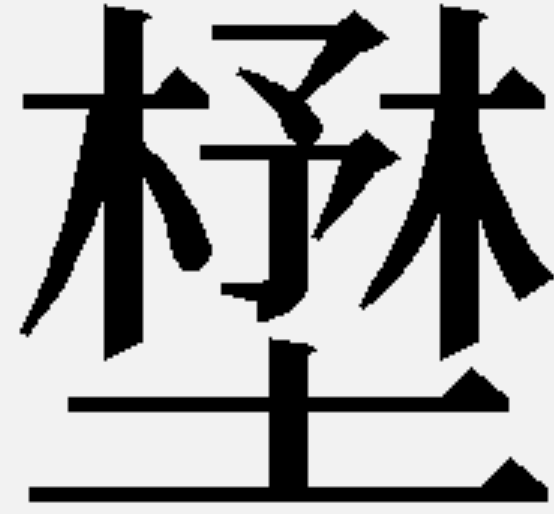
\includegraphics[width=4mm]{U+21428.png}}, and 埜.}	%ye3	
{\large{\textsuperscript{vic·}la}},
\textit{yiaeX};	%yaeX	0083l
{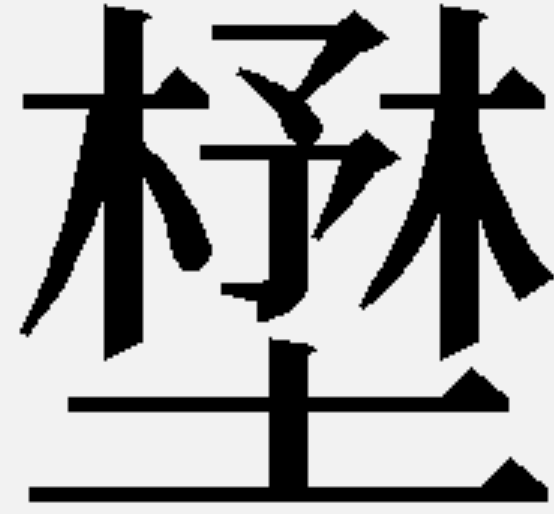
\includegraphics[width=4mm]{U+21428.png}}
{\large{\textsuperscript{vic·}la}},
	%ye3	
%⿱㮊土
\textit{yiaeX};	%yaeX	0083m
埜	%ye3	
{\large{\textsuperscript{vic·}la}},
\textit{yiaeX}.	%yaeX	0083n



\paragraph{\textoversetlarge{01-44}{\huge{兔}}}	
%兔	%tu4	
{\large{ta}},
\textit{thuH};	%thuH	0063a
菟	%tu2	
{\large{\textsuperscript{herb:}ta}},
\textit{du};	%du	0063c


\paragraph{\textoversetlarge{01-45}{\huge{舁}}}	
%舁	%yu2	
\textit{yiəX};	%yoX	0089a
\begin{itemize}
    \item 
{\Large{與}}	{\large{{xxx\textsuperscript{χmolar}}}} = yyy,
%與	%yu2	
\textit{yiə},	%yo	0089b
%與	%yu4	
\textit{yiəH},	%yoH	0089b
%與	%yu3	
\textit{yiəX};	%yoX	0089b
歟	%yu2	
\textit{yiə};	%yo	0089e
璵	%yu2	
\textit{yiə};	%yo	0089f
䑂	%yu3?	
\textit{yiəX};	%yoX	0089g
譽	%yu4	
\textit{yiə},	%yo	0089i
%譽	%yu4	
\textit{yiəH};	%yoH	0089i
輿	%yu2	
\textit{yiə};	%yo	0089j
鸒	%yu4	
\textit{yiəH};	%yoH	0089k
旟	%yu2	
\textit{yiə};	%yo	0089l
藇	%yu3	
\textit{yiəX},	%yoX	0089n
%藇	%xu4	
\textit{ziəX};	%zjoX	0089n
鱮	%xu4	
\textit{ziəX}.	%zjoX	0089o
\end{itemize}

I find this a hard one, because I do not see how we can decide between l- or q-, or y- for that matter. Probably better to use y- to be agnostic. 




\paragraph{\textoversetlarge{01-48}{\huge{舍}}}	
%舍	%she4	
\textit{śiaeH};	%syaeH	0048a
舍	%she3	
\textit{śiaeX};	%syaeX	0048a
捨	%she3	
\textit{śiaeX};	%syaeX	0048c

\paragraph{\textoversetlarge{01-49}{\huge{鼠}}}	
%鼠	%shu3	
\textit{śiəX};	%syoX	0092a
癙	%shu3	
\textit{śiəX};	%syoX	0092b


\paragraph{\textoversetlarge{01-50}{\huge{黍}}}	
%黍	%shu3	
\textit{śiəX};	%syoX	0093a


\paragraph{\textoversetlarge{01-52}{\huge{魯}}}	
%魯	%lu3	
\textit{luX};	%luX	0070a
櫓	%lu3	
\textit{luX};	%luX	0070e

\paragraph{\textoversetlarge{01-53}{\huge{鹵}}}	
%鹵	%lu3	
\textit{luX};	%luX	0071a

\begin{spacing}{0.7} 
\paragraph{\textoversetlarge{01-54}{\huge{呂}}}	
 {\large{r\textoverset{b}{a}}}, 
%呂	%lü3	
\textit{liəX};	%ljoX	0076a
侶	%lü3	
 {\large{{\textsuperscript{hom·}}r\textoverset{b}{a}}}, 
\textit{liəX};	%ljoX	0076d
梠	%lü3	
 {\large{{\textsuperscript{arb·}}r\textoverset{b}{a}}}, 
\textit{liəX};	%ljoX	0076e
閭	%lü2	
 {\large{{\textsuperscript{port:}}r\textoverset{b}{a}}}, 
\textit{liə};	%ljo	0076g
郘	%lü3	
 {\large{r\textoverset{b}{a}{\textsuperscript{·tum}}}}, 
\textit{liəX};	%ljoX	0076h
筥	%ju3	
 {\large{{\textsuperscript{bamb:}}r\textoverset{b}{a}}}, 
\textit{kiəX};	%kjoX	0076j
莒	%ju3	
 {\large{{\textsuperscript{herb:}}r\textoverset{b}{a}}}, 
\textit{kiəX}.	%kjoX	0076l
\end{spacing}

\paragraph{\textoversetlarge{01-55}{\huge{旅}}}	
{\large{ra}},
%旅	%lü3	
\textit{liəX};	%ljoX	0077a
膂	%lü3	
{\large{ra{\textsuperscript{:carn}}}}, 
\textit{liəX};	%ljoX	0077e
玈	%lu2	
 {\large{{\textsuperscript{profund·}}ra}},  
\textit{lu};	%lu	0077f


\begin{spacing}{0.7} 
\paragraph{\textoversetlarge{01-56}{\huge{女}}}	
{\large{na}},
%女	%nü4	
\textit{ṇiəH},	%nrjoH	0094a
%女	%nü3	
\textit{ṇiəX};	%nrjoX	0094a
籹	%nü3	
{\large{\textsuperscript{oryz·}na}},
\textit{ṇiəX};	%nrjoX	0094f
汝	%ru3	
{\large{\textsuperscript{aq·}na}},
\textit{ñiəX};	%nyoX	0094j
\begin{itemize}[noitemsep]
    \item 
    {\Large{如}}	%ru2	
{\large{na\textsuperscript{·or}}} =
{\large{n\textoverset{b}{a}}},
\textit{ñiə};	%nyo	0094g
帤	%ru2	
{\large{n\textoverset{b}{a}\textsuperscript{:lint}}},
\textit{ṇiə};	%nrjo	0094o
袽	%ru2	
{\large{\textsuperscript{vest·}n\textoverset{b}{a}}},
\textit{ṇiə};	%nrjo	0094p
洳	%ru2	
{\large{\textsuperscript{aq·}n\textoverset{b}{a}}},
\textit{ñiə},	%nyo	0094q
%洳	%ru4	
\textit{ñiəH};	%nyoH	0094q
茹	%ru2	
{\large{\textsuperscript{herb·}n\textoverset{b}{a}}},
\textit{ñiə},	%nyo	0094r
%茹	%ru2	
\textit{ñiəH},	%nyoH	0094r
%茹	%ru2	
\textit{ñiəX};	%nyoX	0094r
鴽	%ru2	
{\large{n\textoverset{b}{a}\textsuperscript{:av}}},
\textit{ñiə};	%nyo	0094s
恕	%shu4	
{\large{n\textoverset{b}{a}\textsuperscript{:cor}}},
\textit{śiəH};	%syoH	0094t
絮	%xu4	
{\large{n\textoverset{b}{a}\textsuperscript{:ser}}},
\textit{siəH},	%sjoH	0094u
%絮	%chu4
\textit{ṭhiəH};	%trhjoH	0094u
\item 
{\Large{奴}}	%nu2	
{\large{na\textsuperscript{·dextr}}} = {\large{na₂}}, 
\textit{nu};	%nu	0094l
孥	%nu2	
{\large{na₂:\textsuperscript{fili}}}
\textit{nu};	%nu	0094v
帑	%nu2	
{\large{na₂:\textsuperscript{lint}}},
\textit{nu};	%nu	0094y
弩	%nu3	
{\large{na₂:\textsuperscript{arc}}},
\textit{nuX};	%nuX	0094z
怒	%nu4	
{\large{na₂:\textsuperscript{cor}}},
\textit{nuH},	%nuH	0094a'
%怒	%nu4	
\textit{nuX};	%nuX	0094a'
拏	%na2	
{\large{na₂:\textsuperscript{man}}},
\textit{ṇae};\footnote{Seems to me that 挐	%na2	
\textit{ṇae} should not be included in this series.	
%nrae	0094c' 
}
%nrae	0094b'
砮	%nu3	
{\large{na₂:\textsuperscript{lap}}},
\textit{nu},	%nu	0094d'
%砮	%nu3	
\textit{nuX};	%nuX	0094d'
笯	%nu2	
{\large{\textsuperscript{bamb:}na₂}},
\textit{ṇae},	%nrae	0094e'
%笯	%nu2	
\textit{nu},	%nu	0094e'
%笯	%nu2	
\textit{nuH};	%nuH	0094e'
駑	%nu2	
{\large{na₂:\textsuperscript{equ}}},
\textit{nu}.	%nu	0094f'
\end{itemize}
\end{spacing}


\paragraph{\textoversetlarge{01-57}{\huge{且}}}	
{\large{tsa}},
\textit{tshiaeX},
%且	%ju1	
\textit{tshiə},	%tshjo	0046a
%且	%ju1	
\textit{tsiə};	%tsjo	0046a
罝	%jie1	
{\large{{\textsuperscript{nass:}}tsa}},
\textit{tsiae};	%tsjae	0046h
柤	%zha1	
{\large{{\textsuperscript{arb·}}tsa}},
\textit{tṣae};	%tsrae	0046i
抯	%zha1	
{\large{{\textsuperscript{man·}}tsa}},
\textit{dziaeX},	%dzjaeX	0046j
%抯	%zha1	
\textit{tsiaeX},	%tsjaeX	0046j
%抯	%zha1	
\textit{tṣae};	%tsrae	0046j
蛆	%ju1	
{\large{{\textsuperscript{serp·}}tsa}},
\textit{tsiə};	%tsjo	0046m
岨	%qu1	
{\large{{\textsuperscript{mon·}}tsa}},
\textit{tshiə};	%tshjo	0046n
狙	%ju1	
{\large{{\textsuperscript{can·}}tsa}},
\textit{tshiə};	%tshjo	0046o
疽	%ju1	
{\large{{\textsuperscript{infirm·}}tsa}},
\textit{tshiə};	%tshjo	0046p
砠	%ju1	
{\large{{\textsuperscript{lap·}}tsa}},
\textit{tshiə};	%tshjo	0046q
雎	%ju1	
{\large{tsa{\textsuperscript{·passer}}}},
\textit{tshiə};	%tshjo	0046r
鴡	%ju1	
{\large{tsa{\textsuperscript{·av}}}},
\textit{tshiə};	%tshjo	0046s
苴	%ju1	
{\large{{\textsuperscript{herb:}}tsa}},
\textit{tshiə},	%tshjo	0046t
%苴	%ju1	
\textit{tsiə},	%tsjo	0046t
%苴	%zha3	
\textit{tṣaeX};	%tsraeX	0046t
咀	%ju3	
{\large{{\textsuperscript{or·}}tsa}},
\textit{dziəX};	%dzjoX	0046u
詛	%zu3	
{\large{{\textsuperscript{dic·}}tsa}},
\textit{tṣiəH};	%tsrjoH	0046x
阻	%zu3	
{\large{{\textsuperscript{tum·}}tsa}},
\textit{tṣiəX};	%tsrjoX	0046y
鉏
{\large{{\textsuperscript{met·}}tsa}},
	%zhu4	
\textit{dẓiəX};	%dzrjoX	0046a'
祖	%zu3	
{\large{{\textsuperscript{spirit·}}tsa}},
\textit{tsuX};	%tsuX	0046b'
組	%zu3	
{\large{{\textsuperscript{ser·}}tsa}},
\textit{tsuX};	%tsuX	0046e'
粗	%cu1	
{\large{{\textsuperscript{oryz·}}tsa}},
\textit{dzuX},	%dzuX	0046h'
%粗	%cu1	
\textit{tshu};	%tshu	0046h'
徂	%cu2	
{\large{{\textsuperscript{eo·}}tsa}},
\textit{dzu};	%dzu	0046i'
殂	%cu2	
{\large{{\textsuperscript{mal·}}tsa}},
\textit{dzu};	%dzu	0046j'
駔	%zu4	
{\large{{\textsuperscript{equ·}}tsa}},
\textit{dzuX},	%dzuX	0046m'
%駔	%zang3	
\textit{tsaṅX};	%tsangX	0046m'
楂	%zha1	
\textit{tṣae};	%tsrae	0046u'
\begin{itemize}[noitemsep]
    \item {\Large{租}}	%zu1	
{\large{{\textsuperscript{gran·}}tsa}} = {\large{tsa₂}},
\textit{tsu};	%tsu	0046d'
蒩	%zu1	
\textit{tsu};	%tsu	0046q'
    \item {\Large{沮}}	%ju3	
{\large{{\textsuperscript{aq·}}tsa}} = {\large{tsa₃}},
\textit{dziəX},	%dzjoX	0046k
%沮	%ju4	
\textit{tsiəH};	%tsjoH	0046k
菹	%zu1	
\textit{tṣiə};	%tsrjo	0046n'
\item  
{\Large{助}}	%zhu4	
{\large{tsa{\textsuperscript{·virt}}}}
 = {\large{tsa₄}},
\textit{dẓiəH};	%dzrjoH	0046z
耡	%chu2	
\textit{dẓiə},	%dzrjo	0046o'
%耡	%chu2	
\textit{dẓiəH};	%dzrjoH	0046o'
鋤	%chu2	
\textit{dẓiə};	%dzrjo	0046p'
\item {\Large{虘}}	%cuo2	
{\large{{\textsuperscript{tigr·}}tsa}}   = {\large{tsa₅}},
\textit{dzu};	%dzu	0046k'
%⿰黹虘	%chu3	
{
\includegraphics[width=4.2mm]{U+2A4D0.png}}
{\large{{\textsuperscript{acu·}}tsa}},
\textit{tṣhiəX};	%tsrhjoX	0046r'
樝	%zha1	
\textit{tṣae};	%tsrae	0046s'
{
\includegraphics[width=4.2mm]{U+20B6F.png}}
%⿰虘又	%zha1	
{\large{tsa{\textsuperscript{·dextr}}}},

\textit{tṣae};	%tsrae	0046v'
\end{itemize}


俎	%zu3	
\textit{tṣiəX};	%tsrjoX	0046v
not a XS character



\paragraph{\textoversetlarge{01-58}{\huge{觕}}}	
%觕	%cu1	
\textit{tshu};	%tshu	0065a

\paragraph{\textoversetlarge{01-59}{\huge{麤}}}	
%麤	%cu1	
\textit{tshu};	%tshu	0066a

\paragraph{\textoversetlarge{01-60}{\huge{初}}}	
%初	%chu1	
\textit{tṣhiə};	%tsrhjo	0087a

\paragraph{\textoversetlarge{01-61}{\huge{素}}}	
%素	%su4	
\textit{suH};	%suH	0068a

\begin{spacing}{0.7} 
\paragraph{\textoversetlarge{01-62}{\huge{疋}}}	
{\large{sr\textoverset{b}{a}}},
%疋	%shu1	
\textit{ṣiə};	%srjo	0090a
疎	%shu1	
\textit{ṣiə};	%srjo	0090c
楚
%楚	%chu3	
{\large{\textsuperscript{silv:}sr\textoverset{b}{a}}},
\textit{tṣhiəX};	%tsrhjoX	0088a
\begin{itemize}
    \item {\Large{疏}} 	 %shu1	
{\large{sr\textoverset{b}{a}}} = {\large{sr\textoverset{b}{a}₂}},
\textit{ṣiə};	%srjo	0090b
蔬	%shu1	
\textit{ṣiə};	%srjo	0090d
    \item {\Large{胥}}	%xu1	
{\large{sr\textoverset{b}{a}}} = {\large{sra}},
\textit{siə};	%sjo	0090e
湑	%xu3	
\textit{siəX};	%sjoX	0090f
稰	%xu1	
\textit{siəX};	%sjoX	0090g
糈	%xu3	
\textit{ṣiəX};	%srjoX	0090h
壻	%xu4	
\textit{seyH}.	%sejH	0090i
\end{itemize}
I prefer {\large{sr\textoverset{b}{a}}}
 despite 壻	%xu4	
\textit{seyH}, but maybe this is not valid. 
\end{spacing}


 




\paragraph{\textoversetlarge{01-63}{\huge{所}}}	
%所	%suo3	
\textit{ṣiəX},	%srjoX	0091a
%所	%suo3	
\textit{hiəX};	%xjoX	0091a



\paragraph{\textoversetlarge{01-64}{\huge{普}}}	
%普	%pu3	
\textit{phuX};	%phuX	0072a

\paragraph{\textoversetlarge{01-65}{\huge{步}}}	
%步	%bu4	
\textit{buH};	%buH	0073a

\begin{spacing}{0.7} 
\paragraph{\textoversetlarge{01-66}{\huge{夫}}}	{\large{p\textoverset{b}{a}}}, 
%夫	%fu2	
\textit{biu}	%bju	0101a
%夫	%fu1	
\textit{piu};	%pju	0101a
鈇	%fu1	
{\large{{\textsuperscript{met·}}p\textoverset{b}{a}}},
\textit{piu}	%pju	0101e
%鈇	%fu3	
\textit{piuX};	%pjuX	0101e
扶	%fu2	
{\large{{\textsuperscript{man·}}p\textoverset{b}{a}}},
\textit{biu},	%bju	0101f
%扶	%fu2	
\textit{phu},	%phu	0101f
%扶	%fu2	
\textit{piu};	%pju	0101f
枎	%fu2	
{\large{{\textsuperscript{arb·}}p\textoverset{b}{a}}},
\textit{biu};	%bju	0101g
芙	%fu2	
{\large{{\textsuperscript{herb·}}p\textoverset{b}{a}}},
\textit{biu}.	%bju	0101h
\end{spacing}

\begin{spacing}{0.7} 
\paragraph{\textoversetlarge{01-67}{\huge{父}}}{\huge{(}}{
\includegraphics[width=6mm]{父.png}}{\huge{)}}
%父	%fu4	
{\large{pa}}, 
\textit{biuX},	%bjuX	0102a
%父	%fu3	
\textit{piuX};	%pjuX	0102a
釜	%fu3	
{\large{pa{\textsuperscript{:met}}}},
\textit{biuX};	%bjuX	0102f
斧	%fu3	
{\large{pa{\textsuperscript{:libra}}}},
\textit{piuX};	%pjuX	0102h
\begin{itemize}[noitemsep]
    \item 
{\Large{布}}({
\includegraphics[width=5mm]{布.png}})	%bu4	
{\large{pa{\textsuperscript{:lint}}}} = {\large{p\textoverset{a}{a}}},
\textit{puH};	%puH	0102j
怖	%bu4	
{{\textsuperscript{cor·}}p\textoverset{a}{a}}, 
\textit{phuH};	%phuH	0102m
    \item {\Large{甫}}({
\includegraphics[width=5mm]{甫.png}})	%bu4	
{\large{pa{\textsuperscript{:ager}}}} = {\large{pa₂}},
%fu3	
\textit{piuX};	%pjuX	0102n
脯	%fu3	
{\large{{\textsuperscript{carn·}}pa₂}},
\textit{piuX};	%pjuX	0102r
莆	%fu3	
{\large{{\textsuperscript{herb:}}pa₂}},
\textit{piuX};	%pjuX	0102s
黼	%fu3	
{\large{{\textsuperscript{acu·}}pa₂}},
\textit{piuX};	%pjuX	0102t
簠	%fu3	
{\large{{\textsuperscript{bamb:}}pa₂}},
\textit{piu}, %pju	0102u
%簠	%fu3	
\textit{piuH},	%pjuH	0102u
%簠	%fu3	
\textit{piuX};	%pjuX	0102u
輔	%fu3	
{\large{{\textsuperscript{vehic·}}pa₂}},
\textit{biuX};	%bjuX	0102v
鬴	%fu3	
{\large{{\textsuperscript{olla·}}pa₂}},
\textit{biuX};	%bjuX	0102y
圃	%pu3	
{\large{{\textsuperscript{cla·}}pa₂}},
\textit{puH},	%puH	0102z
%圃	%pu3	
\textit{puX};	%puX	0102z
補	%bu3	
{\large{{\textsuperscript{vest·}}pa₂}},
\textit{puX};	%puX	0102c'
逋	%bu1	
{\large{{\textsuperscript{amb·}}pa₂}},
\textit{pu};	%pu	0102d'
餔	%bu1	
{\large{{\textsuperscript{ed·}}pa₂}},
\textit{pu};	%pu	0102e'
痡	%pu1	
{\large{{\textsuperscript{infirm·}}pa₂}},
\textit{phiu},	%phju	0102g'
%痡	%pu1	
\textit{phu};	%phu	0102g'
鋪	%fu1	
{\large{{\textsuperscript{met·}}pa₂}},
\textit{phiu},	%phju	0102h'
%鋪	%pu1	
\textit{phu};	%phu	0102h'
哺	%bu3	
{\large{{\textsuperscript{or·}}pa₂}},
\textit{buH},	%buH	0102i'
酺	%pu2	
{\large{{\textsuperscript{vin·}}pa₂}},
\textit{bu},	%bu	0102k'
%酺	%pu2	
\textit{buH};	%buH	0102k'
匍	%pu2	
{\large{pa₂{\textsuperscript{·flect}}}},
\textit{bu};	%bu	0102l'
\begin{itemize}
\item 
{\Large{浦}}	
{\large{{\textsuperscript{aq·}}pa₂}} = {\large{p\textoverset{a}{a}₂}},
%pu3	
\textit{phuX};	%phuX	0102f'
蒲	%pu2	
{\large{{\textsuperscript{herb:}}p\textoverset{a}{a}₂}},
\textit{bu};	%bu	0102n'
\item 
{\Large{捕}}	%bu3	
{\large{{\textsuperscript{man·}}pa₂}} = {\large{p\textoverset{a}{a}₃}},
\textit{buH};	%buH	0102j'
蒱	%pu2	
{\large{\textsuperscript{herb:}p\textoverset{a}{a}₃}},
\textit{bu};	%bu	0102o'
\item {\Large{尃}}	%fu1	
{\large{pa₂{\textsuperscript{:digit}}}} = {\large{p\textoverset{b}{a}}},
\textit{phiu};	%phju	0102p'
傅	%fu4	
{\large{{\textsuperscript{hom·}}p\textoverset{b}{a}}}, 
\textit{biuH},	%bjuH	0102u'
%傅	%fu4	
\textit{piuH};	%pjuH	0102u'
榑	%fu2	
{\large{{\textsuperscript{arb·}}p\textoverset{b}{a}}}, 
\textit{biu};	%bju	0102v'
賻	%fu4	
{\large{{\textsuperscript{conch·}}p\textoverset{b}{a}}}, 
\textit{biuH}.	%bjuH	0102x'
\item 旉	%fu1	
{\large{pa₂{\textsuperscript{:quadr}}}} = {\large{p\textoverset{b}{a}₂}},
\textit{phiu};	%phju	0102q'
敷	%fu1	
{\large{p\textoverset{b}{a}₂}{\textsuperscript{·fer}}}, 
\textit{phiu};	%phju	0102t'
\end{itemize}
\end{itemize}
\end{spacing}
The \textit{xiéshēng} analysis of 簠 is not clear to me. 


\begin{spacing}{0.7}
\paragraph{\textoversetlarge{01-68}{\huge{巴}}}	
{\large{pr\textoverset{a}{a}}},
%巴	%ba1	
\textit{pae};	%pae	0039a
把	%ba3	
{\large{{\textsuperscript{man·}}pr\textoverset{a}{a}}},
\textit{paeX};	%paeX	0039b
芭	%ba1	
{\large{\textsuperscript{bamb:}pr\textoverset{a}{a}}},
\textit{pae};	%pae	0039c
豝	%ba1	
{\large{{\textsuperscript{porc·}}pr\textoverset{a}{a}}},
\textit{pae};	%pae	0039d
杷	%pa2	
{\large{{\textsuperscript{arb·}}pr\textoverset{a}{a}}},
\textit{bae};	%bae	0039e
耙	%pa2	
{\large{{\textsuperscript{aratr·}}pr\textoverset{a}{a}}},
\textit{bae},	%bae	0039e
%杷	%ba4	
\textit{baeH}.	%baeH	0039e
%耙	%ba4	
%\textit{baeH};	%baeH	0039e
\end{spacing}

\paragraph{\textoversetlarge{01-69}{\huge{無}}}	{\large{ma}}, 
%無	%wu2	
\textit{miu};	%mju	0103a
廡	%wu3	
{\large{{\textsuperscript{caut·}}ma}},
\textit{miuX};	%mjuX	0103i
憮	%wu3	
{\large{{\textsuperscript{cor·}}ma}},
\textit{miuX},	%mjuX	0103j
%憮	%wu3	
\textit{hu};	%xu	0103j
甒	%wu3	
{\large{ma}{\textsuperscript{·teg}}},
\textit{miuX};	%mjuX	0103k
蕪	%wu2	
{\large{{\textsuperscript{herb·}}ma}},
\textit{miu};	%mju	0103l
譕	%mu2	
{\large{{\textsuperscript{dic·}}ma}},
\textit{miu};	%mju	0103m
幠	%hu1	
{\large{{\textsuperscript{lint·}}ma}},
\textit{hu};	%xu	0103n
膴	%wu2	
{\large{{\textsuperscript{carn·}}ma}},
\textit{miu},	%mju	0103o
%膴	%hu1	
\textit{hiuX},	%xjuX	0103o
%膴	%hu1	
\textit{hu};	%xu	0103o
撫	%fu3	
{\large{{\textsuperscript{man·}}ma}},
\textit{phiuX};	%phjuX	0103p
鄦	%xu3	
{\large{ma{\textsuperscript{·urb}}}},
\textit{hiəX}.	%xjoX	0103q
\begin{itemize}
    \item 舞	%wu3	
{\large{ma{\textsuperscript{·舛}}}}, 
\textit{miuX};	%mjuX	0103g
儛	%wu3	
\textit{miuX};	%mjuX	0103h
\end{itemize}



\begin{spacing}{0.7}
\paragraph{\textoversetlarge{01-73}{\huge{馬}}}	
{\large{mr\textoverset{a}{a}}},
%馬	%ma3	
\textit{maeX};	%maeX	0040a
禡	%ma4	
{\large{{\textsuperscript{spirit·}}mr\textoverset{a}{a}}},
\textit{maeH};	%maeH	0040f
罵	%ma4	
{\large{{\textsuperscript{nass·}}mr\textoverset{a}{a}}},
\textit{maeH},	%maeH	0040h
%罵	%ma4	
\textit{maeX}.	%maeX	0040h
\end{spacing}







\begin{spacing}{0.7} 
\paragraph{\textoversetlarge{02-07}{\huge{䀠}}}	{\large{ku\textoverset{b}{a}}}, 
%䀠	%qu2	
\textit{kiuH};	%kjuH	0096a
\begin{itemize}[noitemsep]
    \item 
{\Large{瞿}}	%qu2	
{\large{gu\textoverset{b}{a}}},
\textit{giu};	%gju	0096c
衢	%qu2	
\textit{giu};	%gju	0096d
躣	%qu2	
\textit{giu};	%gju	0096e
鸜	%qu2	
\textit{giu};	%gju	0096g
臞	%qu2	
\textit{giu},	%gju	0096h
%臞	%qu2	
\textit{giuH};	%gjuH	0096h
懼	%ju4	
\textit{giu};	%gju	0096i
\end{itemize}
\end{spacing}

\paragraph{\textoversetlarge{01-26}{\huge{雨}}}	
%{\large{xx\textoverset{x}{x}}}, 
%雨	%yu4	
\textit{ḫiuH},	%hjuH	0100a
%雨	%yu3	
\textit{ḫiuX},	%hjuX	0100a




\paragraph{\textoversetlarge{01-70}{\huge{无}}}	{\large{xx\textoverset{x}{x}}}, 
无	%wu2	
\textit{miu}.	%mju	0106a


\begin{spacing}{0.7} 
\paragraph{\textoversetlarge{01-71}{\huge{武}}}	{\large{m\textoverset{b}{a}}}, 
%武	%wu3	
\textit{miuX};	%mjuX	0104a
鵡	%wu3	
\textit{miuX};	%mjuX	0104f
賦	%fu4	
\textit{piuH}.	%pjuH	0104g
\end{spacing}
Relevant article by Boltz. 


\paragraph{\textoversetlarge{01-72}{\huge{巫}}}	{\large{xx\textoverset{x}{x}}}, 
	%wu1	
\textit{miu};	%mju	0105a
誣	%wu1	
\textit{miu}.	%mju	0105b


\paragraph{\textoversetlarge{04-64}{\huge{毋}}}	{\large{xx\textoverset{x}{x}}}, 
%wu2	
\textit{miu}.	%mju	0107a

\begin{spacing}{0.7} 
\paragraph{\textoversetlarge{10-01}{\huge{句}}}	{\large{ko}}, 
句	%ju4	
\textit{kiuH},	%kjuH	0108a
%句	%gou1	
\textit{kuw};	%kuw	0108a
鉤	%gou1	
{\large{{\textsuperscript{met·}}ko}},
\textit{kuw};	%kuw	0108c
狗	%gou3	
{\large{{\textsuperscript{can·}}ko}},
\textit{kuwX};	%kuwX	0108d
笱	%gou3	
{\large{{\textsuperscript{bamb·}}ko}},
\textit{kuwX};	%kuwX	0108e
耇	%gou3	
{\large{{\textsuperscript{sen·}}ko}},
\textit{kuwX};	%kuwX	0108f
苟	%gou3	
{\large{{\textsuperscript{herb·}}ko}},
\textit{kuwX};	%kuwX	0108h
雊	%gou4	
{\large{ko{\textsuperscript{·passer}}}},
\textit{kuwH};	%kuwH	0108i
怐	%kou4	
{\large{{\textsuperscript{cor·}}ko}},
\textit{khuw};	%khuw	0108j
敂	%kou4	
{\large{{\textsuperscript{fer·}}ko}},
\textit{khuwH},	%khuwH	0108k
%敂	%kou4	
\textit{khuwX};	%khuwX	0108k
袧	%kou1	
{\large{{\textsuperscript{vest·}}ko}},
\textit{khuw};	%khuw	0108l
訽	%gou4	
{\large{{\textsuperscript{dic·}}ko}},
\textit{ḫuwH},	%huwH	0108m
%訽	%gou4	
\textit{huwH},	%xuwH	0108m
%訽	%gou4	
\textit{huwX};	%xuwX	0108m
蚼	%gou3	
{\large{{\textsuperscript{serp·}}ko}},
\textit{huwX};	%xuwX	0108n
枸	%ju3	
{\large{{\textsuperscript{arb·}}ko}},
\textit{kiuX};	%kjuX	0108o
拘	%ju1	
{\large{{\textsuperscript{manu·}}ko}},
\textit{giu},	%gju	0108p
%拘	%ju1	
\textit{kiu},	%kju	0108p
%拘	%gou1	
\textit{kuw};	%kuw	0108p
痀	%ju1	
{\large{{\textsuperscript{infirm·}}ko}},
\textit{kiu};	%kju	0108q
駒	%ju1	
{\large{{\textsuperscript{equ·}}ko}},
\textit{kiu};	%kju	0108r
劬	%qu2	
{\large{ko{\textsuperscript{·virt}}}},
\textit{giu};	%gju	0108t
絇	%qu2	
{\large{{\textsuperscript{ser·}}ko}},
\textit{giu};	%gju	0108u
胊	%qu2	
{\large{{\textsuperscript{carn·}}ko}},
\textit{giu};	%gju	0108v
軥	%qu2	
{\large{{\textsuperscript{vehic·}}ko}},
\textit{giu};	%gju	0108x
鴝	%qu2	
{\large{ko}{\textsuperscript{·av}}},
\textit{giu};	%gju	0108y
竘	%qu3	
{\large{{\textsuperscript{sto·}}ko}},
\textit{khiuX},	%khjuX	0108z
%竘	%kou3	
\textit{khuwX};	%khuwX	0108z
呴	%xu1	
{\large{{\textsuperscript{or·}}ko}},
\textit{hiu},	%xju	0108a'
%呴	%xu4	
\textit{hiuH};	%xjuH	0108a'
姁	%xu3	
{\large{{\textsuperscript{fem·}}ko}},
\textit{hiuX};	%xjuX	0108b'
\begin{itemize}
    \item 昫 
    {\large{{\textsuperscript{sol·}}ko}} = {\large{k\textoverset{b}o}},
\textit{hiuH}; 煦	%xu4	
{\large{ko{\textsuperscript{·ign}}}},
\textit{hiuH},	%xjuH	0108c'
%煦	%xu3	
\textit{hiuX}.	%xjuX	0108c'
\end{itemize}
\end{spacing}

\begin{spacing}{0.7}
\paragraph{\textoversetlarge{10-02}{\huge{冓}}}	{\large{k\textoverset{a}{o}}}, 
%gou4	
\textit{kuwH};	%kuwH	0109a
媾	%gou4	
{\large{{\textsuperscript{fem·}}k\textoverset{a}{o}}}, 
\textit{kuwH};	%kuwH	0109e
搆	%gou4	
{\large{{\textsuperscript{man·}}k\textoverset{a}{o}}}, 
\textit{kuwH};	%kuwH	0109f
構	%gou4	
{\large{{\textsuperscript{arb·}}k\textoverset{a}{o}}}, 
\textit{kuwH};	%kuwH	0109g
溝	%gou1	
{\large{{\textsuperscript{aq·}}k\textoverset{a}{o}}}, 
\textit{kuw};	%kuw	0109h
篝	%gou1	
{\large{{\textsuperscript{herb:}}k\textoverset{a}{o}}}, 
\textit{kuw};	%kuw	0109i
覯	%gou4	
{\large{k\textoverset{a}{o}}{\textsuperscript{·vid}}}, 
\textit{kuwH};	%kuwH	0109j
購	%gou4	
{\large{{\textsuperscript{conch·}}k\textoverset{a}{o}}}, 
\textit{kuwH};	%kuwH	0109k
遘	%gou4	
{\large{{\textsuperscript{amb·}}k\textoverset{a}{o}}}, 
\textit{kuwH}.	%kuwH	0109l
\end{spacing}

\begin{spacing}{0.7} 
\paragraph{\textoversetlarge{10-03}{\huge{口}}}	{\large{kh\textoverset{a}{o}}}, 
%kou3	
\textit{khuwX};	%khuwX	0110a
叩	%kou4	
{\large{kh\textoverset{a}{o}\textsuperscript{·sign}}}, 
\textit{khuwH},	%khuwH	0110d
%叩	%kou3	
\textit{khuwX};	%khuwX	0110d
扣	%kou4	
{\large{\textsuperscript{man·}}kh\textoverset{a}{o}}, 
\textit{khuwH},	%khuwH	0110e
%扣	%kou3	
\textit{khuwX};	%khuwX	0110e
釦	%kou3	
{\large{\textsuperscript{met·}}kh\textoverset{a}{o}}, 
\textit{khuwX};	%khuwX	0110f
\end{spacing}

\paragraph{\textoversetlarge{10-04}{\huge{寇}}}	{\large{xx\textoverset{x}{x}}}, 
	%kou4	
\textit{khuwH}	%khuwH	0111a

\begin{spacing}{0.7} 
\paragraph{\textoversetlarge{10-05}{\huge{后}}}	
{\large{k\textoverset{a}{o}}}, 
%hou4	
\textit{ḫuwH},	%huwH	0112a
%后	%hou4	
\textit{ḫuwX};	%huwX	0112a
逅	%hou4	
{\large{{\textsuperscript{amb·}}k\textoverset{a}{o}}}, 
\textit{ḫuwH};	%huwH	0112c
垢	%gou4	
{\large{{\textsuperscript{terr·}}k\textoverset{a}{o}}}, 
\textit{kuwX};	%kuwX	0112d
姤	%gou4	
{\large{{\textsuperscript{fem·}}k\textoverset{a}{o}}}, 
\textit{kuwH};	%kuwH	0112e
詬	%gou4	
{\large{{\textsuperscript{dic·}}k\textoverset{a}{o}}}, 
\textit{khuwH},	%khuwH	0112f
%詬	%gou4	
\textit{kuwX};	%kuwX	0112f
㖃	%hou4	
{\large{{\textsuperscript{or·}}k\textoverset{a}{o}}}, 
\textit{huwH},	%xuwH	0112g
%㖃	%hou3	
\textit{huwX}.	%xuwX	0112g
\end{spacing}

\begin{spacing}{0.7} 
\paragraph{\textoversetlarge{10-06}{\huge{侯}}}	{\large{g\textoverset{a}{o}}}, 
%hou2	
\textit{ḫuw};	%huw	0113a
候	%hou4	
{\large{{\textsuperscript{hom·}}g\textoverset{a}{o}}}, 
\textit{ḫuwH};	%huwH	0113e
喉	%hou2	
{\large{{\textsuperscript{or·}}g\textoverset{a}{o}}}, 
\textit{ḫuw}; %huw	0113f
猴	%hou2	
{\large{{\textsuperscript{can·}}g\textoverset{a}{o}}}, 
\textit{ḫuw};	%huw	0113g
翭	%hou2	
{\large{{\textsuperscript{plum·}}g\textoverset{a}{o}}}, 
\textit{ḫuw};	%huw	0113h
鍭	%hou2	
{\large{{\textsuperscript{met·}}g\textoverset{a}{o}}}, 
\textit{ḫuw},	%huw	0113i
%鍭	%hou2	
\textit{ḫuwH};	%huwH	0113i
餱	%hou2	
{\large{{\textsuperscript{ed·}}g\textoverset{a}{o}}}, 
\textit{ḫuw}.	%huw	0113j
\end{spacing}

\paragraph{\textoversetlarge{10-07}{\huge{厚}}}	{\large{xx\textoverset{x}{x}}}, 
%hou4	
\textit{ḫuwX}.	%huwX	0114a


\paragraph{\textoversetlarge{10-08}{\huge{後}}}	{\large{xx\textoverset{x}{x}}},
%hou4	
\textit{ḫuwH},	%huwH	0115a
%後	%hou4	
\textit{ḫuwX}.	%huwX	0115a

\paragraph{\textoversetlarge{10-12}{\huge{兜}}}	{\large{xx\textoverset{x}{x}}},
%dou1	
\textit{tuw}.	%tuw	0117a

\end{multicols}

I have left off at GSR 100 


\paragraph{\textoversetlarge{10-09}{\huge{具}}}	{\large{xx\textoverset{x}{x}}},
%ju4	
\textit{giuH};	%gjuH	0121a
俱	%ju4	
\textit{kiu}; %kju	0121d
椇	%ju3	
\textit{kiuX}.	%kjuX	0121e

\paragraph{\textoversetlarge{10-10}{\huge{區}}}	{\large{q\textoverset{x}{o}}},
%ou1	
\textit{{\sil{ꞏ}}uw},	%'uw	0122a
%區	%qu1	
\textit{khiu};	%khju	0122a
驅	%qu1	
{\large{{\textsuperscript{equ·}}q\textoverset{x}{o}}},
\textit{khiu},	%khju	0122c
%驅	%qu1	
\textit{khiuH};	%khjuH	0122c
敺	%qu1	
{\large{q\textoverset{x}{o}}{\textsuperscript{·fer}}}, 
\textit{khiu},	%khju	0122d
%敺	%qu4	
\textit{khiuH};	%khjuH	0122d
軀	%qu1	
{\large{{\textsuperscript{corp·}}q\textoverset{x}{o}}}, 
\textit{khiu},	%khju	0122g
%軀	%qu1	
\textit{khiuH};	%khjuH	0122g
摳	%kou1	
{\large{{\textsuperscript{man·}}q\textoverset{x}{o}}}, 
\textit{khiu},	%khju	0122h
%摳	%kou1	
\textit{khuw};	%khuw	0122h
嘔	%ou1	
{\large{{\textsuperscript{or·}}q\textoverset{x}{o}}}, 
\textit{{\sil{ꞏ}}uw},	%'uw	0122i
%嘔	%ou3	
\textit{{\sil{ꞏ}}uwX};	%'uwX	0122i
毆	%ou3	
{\large{q\textoverset{x}{o}}{\textsuperscript{·hast}}}, 
\textit{{\sil{ꞏ}}uwX};	%'uwX	0122j
漚	%ou1	
{\large{{\textsuperscript{aq·}}q\textoverset{x}{o}}}, 
\textit{{\sil{ꞏ}}uw},	%'uw	0122k
%漚	%ou4	
\textit{{\sil{ꞏ}}uwH};	%'uwH	0122k
甌	%ou1	
{\large{q\textoverset{x}{o}}{\textsuperscript{·teg}}}, 
\textit{{\sil{ꞏ}}uw};	%'uw	0122l
謳	%ou1	
{\large{{\textsuperscript{dic·}}q\textoverset{x}{o}}}, 
\textit{{\sil{ꞏ}}uw};	%'uw	0122m
傴	%yu3	
{\large{{\textsuperscript{hom·}}q\textoverset{x}{o}}}, 
\textit{{\sil{ꞏ}}iuX};	%'juX	0122n
嫗	%yu4	
{\large{{\textsuperscript{fem·}}q\textoverset{x}{o}}}, 
\textit{{\sil{ꞏ}}iuH},	%'juH	0122o
%嫗	%yu3	
\textit{{\sil{ꞏ}}iuX};	%'juX	0122o
饇	%yu4	
{\large{{\textsuperscript{ed·}}q\textoverset{x}{o}}}, 
\textit{{\sil{ꞏ}}iuH},	%'juH	0122p
%樞	%shu1	
\textit{{\sil{ꞏ}}uw};	%'uw	0122q
樞	%shu1	
{\large{q\textoverset{x}{o}}}, 
\textit{chiu};	%tsyhu	0122q
貙	%chu1	
{\large{q\textoverset{x}{o}}}, 
\textit{ṭhiu}.	%trhju	0122r

\paragraph{\textoversetlarge{10-11}{\huge{禺}}}	{\large{ṅo}}, 
%yu2	
\textit{ṅiu},	%ngju	0124a
%禺	%yu4	
\textit{ṅiuH};	%ngjuH	0124a
寓	%yu4	
{\large{{\textsuperscript{tect:}}ṅo}}, \textit{ṅiuH};	%ngjuH	0124c
嵎	%yu2	
{\large{{\textsuperscript{mon·}}ṅo}}, \textit{ṅiu};	%ngju	0124f
愚	%yu2	
{\large{ṅo{\textsuperscript{:cor}}}}, 
\textit{ṅiu};	%ngju	0124g
遇	%yu4	
{\large{ṅo}}, \textit{ṅiuH};	%ngjuH	0124h
隅	%yu2	
{\large{{\textsuperscript{tum·}}ṅo}}, \textit{ṅiu};	%ngju	0124i
腢	%ou3	
{\large{{\textsuperscript{carn·}}ṅo}}, \textit{ṅiu},	%ngju	0124j
%腢	%ou3	
\textit{ṅuwX};	%nguwX	0124j
髃	%yu2	
{\large{{\textsuperscript{oss·}}ṅo}},  \textit{ṅiu},	%ngju	0124k
%髃	%ou3	
\textit{ṅuwX};	%nguwX	0124k
齵	%yu2	
{\large{{\textsuperscript{dent·}}ṅo}}, 
\textit{ṅiu},	%ngju	0124l
%齵	%ou2	
\textit{ṅuw};	%nguw	0124l
喁	%yong2	
{\large{{\textsuperscript{or·}}ṅo}},
\textit{ṅiəwṅ},	%ngjowng	0124m
%喁	%yu2	
\textit{ṅiu},	%ngju	0124m
%喁	%yong2	
\textit{ṅuwX};	%nguwX	0124m
偶	%ou3	
{\large{{\textsuperscript{hom·}}ṅo}},
\textit{ṅuwH},	%nguwH	0124n
%偶	%ou3	
\textit{ṅuwX};	%nguwX	0124n
耦	%ou3	
{\large{{\textsuperscript{aratr·}}ṅo}},
\textit{ṅuwX};	%nguwX	0124o
顒	%yong2	
{\large{ṅo{\textsuperscript{·fac}}}},
\textit{ṅiəwṅ}.	%ngjowng	0124p

The contact between open syllable and velar nasal final in this series is super weird. 

\paragraph{\textoversetlarge{10-13}{\huge{斗}}}	{\large{to}},
%zhu3	
\textit{ciuX},	%tsyuX	0116a
%斗	%dou3	
\textit{tuwX};	%tuwX	0116a
枓	%zhu3	
{\large{{\textsuperscript{arb·}}to}},
\textit{ciuX}.	%tsyuX	0116b

\paragraph{\textoversetlarge{10-16}{\huge{豆}}}	{\large{to}},
%dou4	
\textit{duwH};	%duwH	0118a
脰	%dou4	
{\large{{\textsuperscript{luna·}}to}},
\textit{duwH};	%duwH	0118d
頭	%tou2	
{\large{to{\textsuperscript{·fac}}}},
\textit{duw};	%duw	0118e
裋	%shu4	
{\large{{\textsuperscript{vest·}}to}},
\textit{jiuX};	%dzyuX	0118f
豎	%shu4	
{\large{{\textsuperscript{firm:}}to}},
\textit{jiuX}.	%dzyuX	0118g

\paragraph{\textoversetlarge{10-18}{\huge{朱}}}	{\large{xx\textoverset{x}{x}}},
%zhu1	
\textit{ciu};	%tsyu	0128a
侏	%zhu1	
\textit{ciu};	%tsyu	0128d
珠	%zhu1	
\textit{ciu};	%tsyu	0128e
株	%zhu1	
\textit{ṭiu};	%trju	0128f
蛛	%zhu1	
\textit{ṭiu};	%trju	0128g
鼄	%zhu1	
\textit{ṭiu};	%trju	0128h
誅	%zhu1	
\textit{ṭiu};	%trju	0128k
跦	%zhu1	
\textit{ṭiu};	%trju	0128l
邾	%zhu1	
\textit{ṭiu};	%trju	0128m
姝	%shu1	
\textit{chiu};	%tsyhu	0128p
袾	%chu1	
\textit{chiu},	%tsyhu	0128r
%袾	%zhu1	
\textit{ciu};	%tsyu	0128r
殊	%shu1	
\textit{jiu};	%dzyu	0128s
銖	%zhu1	
\textit{jiu};	%dzyu	0128t
咮	%zhou4	
\textit{ṭiuwH},	%trjuwH	0128u
%咮	%zhou4	
\textit{tuwH}.	%tuwH	0128u

\paragraph{\textoversetlarge{10-19}{\huge{主}}}	{\large{xx\textoverset{x}{x}}},
%zhu3	
ciuX;	%tsyuX	0129a
罜	%zhu3	
ciuH;	%tsyuH	0129b
注	%zhu4	
ṭiuH,	%trjuH	0129c
%注	%zhu4	
ciuH;	%tsyuH	0129c
註	%zhu4	
ṭiuH,	%trjuH	0129d
%註	%zhu4	
ciuH;	%tsyuH	0129d
拄	%zhu3	
ṭiuX	trjuX	0129e
鉒	%zhu4	
ṭiuH	trjuH	0129f
住	%zhu4	
ḍiuH	drjuH	0129g
柱	%zhu4	
ḍiuX	drjuX	0129h
黈	%tou3	
thuwX	thuwX	0129i



\paragraph{\textoversetlarge{10-22}{\huge{壴}}}	{\large{xx\textoverset{x}{x}}},
%zhu3	
ṭiuH;	%trjuH	0127a
尌	%shu4	
jiuH;	%dzyuH	0127h
樹	%shu4	
jiuH;	%dzyuH	0127j
%樹	%shu4	
jiuX;	%dzyuX	0127j
廚	%chu2	
ḍiu;	%drju	0127m
躕	%chu2	
ḍiu.	%drju	0127n


\paragraph{\textoversetlarge{10-23}{\huge{俞}}}	{\large{xx\textoverset{x}{x}}},
%yu	
yiu;	%yu	0125a
喻	%yu4	
yiuH;	%yuH	0125c
愈	%yu4	
yiuX;	%yuX	0125d
愉	%yu2	
yiu;	%yu	0125f
榆	%yu2	
yiu;	%yu	0125g
渝	%yu2	
yiu;	%yu	0125h
瑜	%yu2	
yiu;	%yu	0125i
瘉	%yu4	
yiuX;	%yuX	0125j
羭	%yu2	
yiu;	%yu	0125k
覦	%yu2	
yiu,	%yu	0125l
%覦	%yu2	
yiuH;	%yuH	0125l
諭	%yu4	
yiuH;	%yuH	0125m
踰	%yu2	
yiu;	%yu	0125n
逾	%yu2	
yiu;	%yu	0125o
揄	%yu2	
duwX,	%duwX	0125p
%揄	%yu2	
yiu;	%yu	0125p
窬	%yu2	
duw,	%duw	0125q
%窬	%yu2	
yiu;	%yu	0125q
蝓	%yu2	
yiu,	%yu	0125r
%蝓	%yu2	
źiu	dzyu	CHECK RMC EADING 0125r;
輸	%shu1	
śiu;	%syu	0125s
歈	%yu2	
duw;	%duw	0125t
偷	%tou1	
thuw;	%thuw	0125u
媮	%tou1	
thuw.	%thuw	0125v

\paragraph{\textoversetlarge{10-24}{\huge{臾}}}	{\large{xx\textoverset{x}{x}}},
臾	%yu2	
yiu;	%yu	0126a
庾	%yu3	
yiuX;	%yuX	0126b
斞	%yu3	
yiuX;	%yuX	0126c
楰	%yu2	
yiuX;	%yuX	0126d
腴	%yu2	
yiu;	%yu	0126e
諛	%yu2	
yiu;	%yu	0126f
斔	%yu3	
yiuX.	%yuX	0126g


\paragraph{\textoversetlarge{10-27}{\huge{漏}}}	{\large{xx\textoverset{x}{x}}},
%lou4	
\textit{luwH}	%luwH	0120a


\paragraph{\textoversetlarge{10-29}{\huge{婁}}}	{\large{xx\textoverset{x}{x}}},
%lou2	
\textit{liu},	%lju	0123a
%婁	%lou2	
\textit{liuX},	%ljuX	0123a
%婁	%lou2	
\textit{luw};	%luw	0123a
婁	%lou2	
\textit{luwX};	%luwX	0123a
僂	%lü3	
\textit{liuX},	%ljuX	0123b
%僂	%lou2	
\textit{luw};	%luw	0123b
膢	%lü2	
\textit{liu},	%lju	0123c
%膢	%lou2	
\textit{luw};	%luw	0123c
摟	%lou2	
\textit{luw};	%luw	0123d
蔞	%lou2	
\textit{liu},	%lju	0123e
%蔞	%lü3	
\textit{liuX},	%ljuX	0123e
%蔞	%lou2	
\textit{luw};	%luw	0123e
屢	%lü3	
\textit{liuH};	%ljuH	0123f
瘻	%lü2	
\textit{liu};	%lju	0123g
縷	%lü3	
\textit{liuX};	%ljuX	0123h
鞻	%lou2	
\textit{kiuH},	%kjuH	0123i
%鞻	%lou2	
\textit{liuH},	%ljuH	0123i
%鞻	%lou2	
\textit{luw};	%luw	0123i
塿	%lou3	
\textit{luwX};	%luwX	0123j
樓	%lou2	
\textit{luw};	%luw	0123k
螻	%lou2	
\textit{luw},	%luw	0123l
%螻	%lou2	
\textit{luwH};	%luwH	0123l
鏤	%lou4	
\textit{luwH};	%luwH	0123m
髏	%lou2	
\textit{luw};	%luw	0123n
窶	%ju4	
\textit{giuX};	%gjuX	0123o
寠	%ju4	
\textit{giuX};	%gjuX	0123p
屨	%ju4	
\textit{kiuH};	%kjuH	0123q
數	%shu4	
\textit{ṣiuH},	%srjuH	0123r
%數	%shu3	
\textit{ṣiuX}.	%srjuX	0123r


\paragraph{\textoversetlarge{10-33}{\huge{走}}}	{\large{xx\textoverset{x}{x}}},
%zou3	
\textit{tsuwX}	%tsuwX	0119a




\paragraph{\textoversetlarge{02-30}{\huge{若}}}	{\large{nak}},
%若	%ruo4	
\textit{ñiak};	%nyak	0777a
諾	%nuo4	
{\large{\textsuperscript{dic·}nak}},
\textit{nak};	%nak	0777f
箬	%ruo4	
{\large{\textsuperscript{bamb·}nak}},
\textit{ñiak};	%nyak	0777g
鄀	%ruo4	
{\large{nak\textsuperscript{·urb}}},
\textit{ñiak};	%nyak	0777i
婼	%chuo4	
{\large{\textsuperscript{fem·}nak}},
\textit{ṭhiak};	%trhjak	0777k
\begin{itemize}
    \item 匿	%ni4	
{\large{\textsuperscript{latebrχ}nak}} = 
{\large{nək}},
\textit{ṇik};	%nrik	0777l
暱	%ni4	
{\large{\textsuperscript{sol·}nək}},
\textit{ṇik};	%nrik	0777n
慝	%te4	
{\large{nək\textsuperscript{:cor}}},
\textit{thək}.	%thok	0777o

\end{itemize}


\paragraph{\textoversetlarge{13-26}{\huge{周}}}	
{\large{tiw}},
\textit{ciuw},	%tsyuw	1083a
%周	%zhou1	
\textit{ciuwX};	%tsyuwX	1083a
婤	%zhou1	
{\large{\textsuperscript{fem·}tiw}},
\textit{ciuw};	%tsyuw	1083f
賙	%zhou1	
{\large{\textsuperscript{conch·}tiw}},
\textit{ciuw};	%tsyuw	1083h
輖	%zhou1	
{\large{\textsuperscript{vehic·}tiw}},
\textit{ciuw};	%tsyuw	1083i
啁	%zhao1	
{\large{\textsuperscript{or·}tiw}},
\textit{ṭaew},	%traew	1083j
%啁	%zhou1	
\textit{ṭiuw};	%trjuw	1083j
惆	%chou2	
{\large{\textsuperscript{cor·}tiw}},
\textit{ṭhiuw};	%trhjuw	1083k
稠	%chou2	
{\large{\textsuperscript{gran·}tiw}},
\textit{ḍiuw};	%drjuw	1083l
綢	%chou2	
{\large{\textsuperscript{ser·}tiw}},
\textit{ḍiuw};	%drjuw	1083m
裯	%chou2	
{\large{\textsuperscript{vest·}tiw}},
\textit{ḍiuw};	%drjuw	1083n
凋	%diao1	
{\large{\textsuperscript{glac·}tiw}},
\textit{tew};	%tew	1083o
琱	%diao1	
{\large{\textsuperscript{gem·}tiw}},
\textit{tew};	%tew	1083p
彫	%diao1	
{tiw\large{\textsuperscript{·cri}}},
\textit{tew};	%tew	1083r
錭	%diao1	
{\large{\textsuperscript{met·}tiw}},
\textit{tew};	%tew	1083s
雕	%diao1	
{\large{tiw\textsuperscript{·passer}}},
\textit{tew};	%tew	1083t
鵰	%diao1	
{\large{tiw\textsuperscript{·av}}},
\textit{tew};	%tew	1083u
蜩	%tiao2	
{\large{\textsuperscript{serp·}tiw}},
\textit{dew};	%dew	1083v
調	%tiao2	
{\large{\textsuperscript{dic·}tiw}},
\textit{dew};	%dew	1083x
禂	%dao3	
{\large{\textsuperscript{spirit·}tiw}},
\textit{tawX};	%tawX	1083y
倜	%ti4	
{\large{\textsuperscript{hom·}tiw}},
\textit{thek}.	%thek	1083z

\begin{itemize}
    \item 柬 keanX <  *k\textsuperscript{ˤ}r[a]nʔ = Kren
    \item 諫 kaenH < *k\textsuperscript{ˤ}r[a]nʔ-s = \textsuperscript{dic.}Kren
    \item 揀 keanX < *k\textsuperscript{ˤ}r[a]nʔ = \textsuperscript{man.}Kren
    \item 闌 lan < *[r]\textsuperscript{ˤ}an = \textsuperscript{por\textsuperscript{x}}Kren = ran
    \begin{itemize}
        \item 瀾 lan, lanH < *[r]\textsuperscript{ˤ}anʔ = \textsuperscript{aq.}ran
        \item 爛 lanH < *[r]\textsuperscript{ˤ}an-s = \textsuperscript{ign.}ran
        \item 蘭 lan < *k.[r]\textsuperscript{ˤ}an = \textsuperscript{herb:}ran = k.ran
        \begin{itemize}
            \item 爤 lanH < ?*k.[r]\textsuperscript{ˤ}an = \textsuperscript{ign.}k.ran
        \end{itemize}
        \item 讕 lan, lanX < *g.ra:n\footnote{Zhengzhang's reconstruction.} = \textsuperscript{dic.}ran
        \item 欄 lenH < *g.ra:n\footnote{\textit{ibid.}} = \textsuperscript{arb.}ran
    \end{itemize}
    \item 湅 lenH < *g.re:ns\footnote{\textit{ibid.}} = \textsuperscript{aq.}Kren
    \item 練 lenH < *r\textsuperscript{ˤ}en-s = \textsuperscript{ser.}Kren
    \item 鍊 lenH < *r\textsuperscript{ˤ}en-s = \textsuperscript{met.}Kren
\end{itemize}




\end{document}
